% !TEX program = xelatex
\documentclass[withoutpreface]{cumcmthesis}
\usepackage{siunitx}

\title{NIPT 的时点选择与胎儿的异常判定}
\tihao{C}
\baominghao{0000}
\schoolname{上海科技大学}
\membera{}
\memberb{}
\memberc{}
\supervisor{}
\yearinput{2025}
\monthinput{09}
\dayinput{04}

\begin{document}
\maketitle

\begin{abstract}
  非侵入性产前检测(NIPT)作为产前筛查的重要方法,能够通过分析孕妇血浆中的游离DNA片段,在孕早期对胎儿常见染色体异常进行风险评估。其检测准确性在很大程度上依赖于胎儿游离DNA比例(fetal fraction, FF),而孕周与母体BMI等因素均对FF水平产生显著影响。如何在不同孕妇群体中合理确定检测时机并评估检测误差,从而实现结果的稳健性,是NIPT方法推广应用中的关键科学问题。

  本文围绕数学建模竞赛C题所提出的四个问题展开研究:首先,通过回归与相关性分析,建立胎儿Y染色体浓度与孕周、BMI的关系模型,检验变量间的统计显著性;其次,结合BMI分层优化策略,确定不同孕妇群体的合理检测时点,以平衡早期筛查与检测失败风险;进一步地,引入多因素建模与机器学习方法,综合考虑身高、体重、年龄等临床特征以及检测误差,提出个体化的最佳检测时机推荐模型;最后,针对女胎样本无法依赖Y染色体信号的特点,设计了融合Z值统计、测序质量指标与多维特征的异常判定方法,提高常见染色体非整倍体识别的准确性与稳健性。
  
  整体而言,本研究通过回归建模、生存分析与机器学习方法相结合,系统探讨了NIPT中检测时机选择与异常判定的建模思路。所提出的框架不仅在理论上具有可解释性和推广性,也为临床实际应用提供了优化参考,为降低无结果率、提升检测可靠性提供了方法论支持。
\keywords{无创产前检测(NIPT);线性混合效应模型(LMM);自然样条;加速失效时间模型(AFT);Turnbull非参数估计;CART分组;Monte~Carlo稳健性分析}
\end{abstract}

\section{问题重述}
\subsection{背景与目标}
无创产前检测(Non-invasive Prenatal Testing,NIPT)是近年来发展迅速的一项重要产前筛查技术,它通过采集孕妇血液、检测胎儿的游离DNA片段并分析胎儿染色体是否存在异常,从而确定胎儿的健康状况。与传统的羊水穿刺等侵入性检查相比,NIPT具有安全性高、创伤小等优势,在临床产前筛查与诊断领域具有重要意义。

NIPT 的主要检测目标集中在三种疾病:唐氏综合征、爱德华氏综合征和帕陶氏综合征,这三种体征分别由胎儿21号、18号和13号“染色体游离DNA 片段的比例”是否异常决定。NIPT的准确性主要由胎儿性染色体(男胎XY,女胎XX)浓度判断:如果男胎的Y 染色体浓度达到或高于4\%、女胎的X 染色体浓度没有异常,则可认为NIPT 的结果是基本准确的,否则难以保证结果准确性要求。

题目资料中显示:实践表明,男胎Y染色体浓度与孕妇孕周数及其身体质量指数(BMI)紧密相关。由于孕妇存在个体差异,对所有孕妇采用简单的经验分组和统一的检测时点进行NIPT,会对其准确性产生较大影响。因此,本文章依据附件中提供的数据建立数学模型,计算出不同情况下针对男胎最佳的基于BMI的孕妇分组策略、NIPT时点以及女胎异常的判定方法。
\subsection{数据说明}
本文使用的数据均来源于题目中提供的数据表,为某地区(大多为高BMI)孕妇的NIPT 数据。检测方对某些孕妇有多次采血多次检测或一次采血多次检测的情况,增加了检测结果的可靠性。数据主要包含以下指标:孕妇信息(孕妇代码、年龄、身高、体重、末次月经时间、IVF妊娠方式、BMI)、NIPT时点信息(检测时间、检测时的孕周)以及NIPT数据(如原始测序读段数、GC含量、各染色体Z值与浓度等)。

\subsection{问题概述}
题目中要求解答的四个子问题如下:
第一,分析胎儿Y染色体浓度与孕妇孕周数和BMI等指标之间的相关特性,建立量化关系模型,并验证模型的统计显著性。
第二,确定男胎孕妇的BMI分组区间和最佳NIPT时点,并分析检测误差对结果的影响。
第三,综合考虑孕妇的身高、体重、年龄等孕妇个体差异的影响,以及检测误差和胎儿的Y 染色体浓度达标比例,根据BMI进行分组并确定最佳NIPT时点,使孕妇潜在风险最小。
第四,以女胎孕妇的21号、18号和13号染色体非整倍体(AB列)为判定结果,综合考虑X染色体及上述染色体的Z值、GC含量、读段数及相关比例、BMI 等因素,给出女胎异常的判定方法。

\section{模型假设}

为了确保模型构建的逻辑严谨性与可行性,我们提出以下基本假设:

\begin{enumerate}
    \item \textbf{数据代表性假设}:我们假设所提供的 NIPT 数据集,尽管主要覆盖高 BMI 孕妇群体,但在该人群内部能够真实反映胎儿 Y 染色体浓度、孕妇生理指标及测序数据间的统计规律。模型的结论主要适用于与样本数据具有相似基线特征的孕妇群体。
    
    \item \textbf{测量准确性假设}:对于模型的主要构建过程,我们假设 NIPT 检测得到的各项指标(如 Y 染色体浓度、Z 值等)是准确的。这一假设基于实际操作中常采用多次采样或单一样本多次检测的技术手段,这能有效减少随机测量误差(random error)。然而,我们承认潜在的系统误差或残余随机误差依然存在,因此在问题二和问题三的稳健性分析中,我们放宽了此假设,通过 \textbf{蒙特卡洛(Monte Carlo)模拟} 系统地评估了测量误差对决策时点 $w_g^*$ 的影响。
    
    \item \textbf{观测独立性假设}:在构建不考虑个体重复测量的基准模型时(如问题一的普通最小二乘法 OLS 模型),我们假设不同孕妇的观测样本之间是相互独立的。此假设在后续的最终模型中被放宽,我们采用了 \textbf{线性混合效应模型(Linear Mixed-Effects Model)},通过引入随机截距项,明确地对同一孕妇多次测量数据间的相关性进行了建模。
    
    \item \textbf{金标准有效性假设}:在问题四女胎非整倍体异常的分类模型中,我们假设题目数据中提供的 “AB 列” 标签是判定胎儿是否异常的 “金标准”,即其标注是准确无误的。这是构建和评估监督学习模型的必要前提。
    
    \item \textbf{模型框架适用性假设}:在问题二和问题三中,我们采用 \textbf{加速失效时间(Accelerated Failure Time, AFT)模型}。我们假设协变量(如 BMI、年龄等)对事件时间(Y 浓度达标孕周)的影响是通过一个加速因子(acceleration factor)以乘法形式作用于时间尺度。该假设的合理性通过模型拟合优度(AIC 最小)以及与非参数 Turnbull 估计结果的高度一致性得到了验证。
\end{enumerate}

\section{符号说明}

为确保论文的清晰性与准确性,本节对全文使用的主要数学符号、变量及评价指标进行统一说明。

\subsection{符号与变量定义}

下表定义了本文模型中使用的核心符号与变量:

\begin{table}[H]
  \centering
  \renewcommand{\arraystretch}{1.2}
  \begin{tabular}{ll}
  \hline
  \textbf{符号} & \textbf{定义} \\ \hline
  $Y, V$ & 胎儿 Y 染色体浓度(Fetal Y-chromosome Fraction, FFY),取值在 $(0,1)$ \\
  $W$ & 孕周(Gestational Weeks),以周为单位的连续变量 \\
  $B$ & 孕妇身体质量指数(Body Mass Index, BMI),单位为 $kg/m^2$ \\
  $g$ & 孕妇个体的唯一标识符(Patient ID) \\
  $i$ & 观测样本的索引 \\
  $Z_k$ & 第 $k$ 号染色体的 Z 值(Z-score),衡量其偏离正常均值的程度 \\
  $T$ & 事件时间(Time-to-Event),定义为 Y 浓度首次达到 $4\%$ 阈值的孕周 \\
  $(L,R]$ & 区间删失(Interval Censoring)数据中的观测区间 \\
  $G$ & 孕妇的 BMI 分组集合 \\
  $\tau$ & 置信水平(Confidence Level),即要求组内达到 Y 浓度阈值的孕妇比例 \\
  $w_g^*(\tau)$ & 针对 BMI 分组 $g$,在置信水平 $\tau$ 下的 “最早安全 NIPT 孕周” \\
  $S(t \| \mathbf{X})$ & 生存函数,表示在协变量 $\mathbf{X}$ 条件下 $T>t$ 的概率 \\
  $\beta, \gamma, \alpha, \eta$ & 模型的固定效应参数向量 \\
  $u_g$ & 孕妇个体 $g$ 的随机效应,$u_g \sim \mathcal{N}(0,\sigma_u^2)$ \\
  $\varepsilon_i$ & 模型的随机误差项 \\
  $X$ & 特征矩阵,用于分类模型 \\
  $y$ & 目标标签,二分类变量,$y=1$ 表示女胎异常,$y=0$ 表示正常 \\
  $\hat{p}(x)$ & 模型预测样本 $x$ 为异常的概率 \\
  $\tau^\star$ & 分类模型的最优决策阈值(Optimal Decision Threshold) \\ \hline
  \end{tabular}
  \end{table}


\section{模型建立与求解}

\subsection{问题一的建模与求解}
\subsubsection{问题分析}

问题一旨在基于附件所给的母体外周血 NIPT 数据,刻画并检验“胎儿 Y 染色体浓度(记为 $V$)—孕周(weeks)—BMI”之间的统计关联关系,构建可解释且稳健的关系模型,并对其显著性与拟合优度进行系统评估,从而为问题二与问题三中的时点选择与分组优化提供量化依据。数据来源于竞赛附件(包含孕周、BMI、测序质量与重复检测信息等),研究中将遵循基本的质量控制与清洗流程,对异常时点、测序质量异常、非整倍体标记样本、缺失与极值进行规范化处理,并在存在多次检测的情况下遵循“个体为单位”的处理原则以避免统计依赖带来的偏差。

随后,为形成初步认识并校准建模假设,将开展探索性数据分析与可视化,包括对 $V$、weeks 与 BMI 的分布刻画、散点图与平滑趋势对比、BMI 分层下的趋势检视,以及相关性与描述性统计的归纳。该步骤的目标是识别潜在的线性或非线性关系、评估异方差与长尾特征,并观察是否存在可解释的交互迹象,为后续模型族的选择与对比提供证据。

接下来,在建模与检验层面,将以多层次的策略推进:以线性回归作为基准,进而考虑非线性效应(如对 weeks 引入自然样条/广义可加式结构)以刻画可能的曲线增长趋势;鉴于同一受试者可能存在重复测量,将引入混合效应框架并设置随机截距(必要时评估随机斜率)以处理个体内相关;同时,针对测序数据常见的方差不齐与误差结构,采用稳健推断(如异方差稳健标准误)与残差诊断保证结论的可靠性。在模型优选与稳健性评估中,将综合使用信息准则(AIC/BIC)、似然比检验、交叉验证与残差/影响诊断,确认 weeks 与 BMI 的主效应方向、显著性及其可能的非线性成分是否成立,并据此确定最终推荐模型。

最后,结果呈现将聚焦于两类输出:一是对“孕周与 BMI 对 $V$ 的显著影响及其函数形态”的总体性结论与可视化证据;二是与临床实践相关的判定信息(如达到可靠阈值的概率地图与分层解读),为问题二与问题三中的最佳时点选择与分组方案提供直接的模型基础与量化支撑。问题一的思维框架如下图所示:

\subsubsection{数据预处理}
在本问题中,根据需要,数据预处理主要包括以下步骤:首先进行变量解析与转换,如将孕周转换为数值($"11w+6" → 11.857$),并将BMI转换为浮点数。其次,为保证结果的准确性,我们根据以下标准对数据进行过滤:仅保留10-25周的样本;要求GC含量在40\%-60\%范围内;剔除13/18/21号染色体为非整倍体的样本;并排除关键变量(孕周数, BMI, Y浓度)缺失的记录。
数据清洗后,最终分析样本量为555个,来自242名孕妇,其中76.9\%的孕妇有重复测量记录,平均测量次数为2.29次/人。

\subsubsection{模型的建立}
\paragraph{变量与参数定义}
设响应变量为胎儿Y染色体浓度 $Y\in(0,1)$,自变量包括孕周 $W$ 与体质指数 $B$(BMI),个体标识为患者ID记为 $g$。为用于临床阈值判定,定义二分类变量 $Z=\mathbb{I}(Y\ge 0.04)$。

基线线性回归形式为
\[
Y_i=\beta_0+\beta_W W_i+\beta_B B_i+\varepsilon_i,
\]
其中 $\varepsilon_i$ 为均值为0的误差项。考虑孕周的非线性效应,引入自然样条基 $\mathbf{s}(W_i;df=3)$,得到
\[
Y_i=\beta_0+\mathbf{s}(W_i)^\top\boldsymbol{\gamma}+\beta_B B_i+\varepsilon_i.
\]
为处理重复测量的聚类结构,引入随机截距 $u_{g(i)}\sim\mathcal{N}(0,\sigma_u^2)$:
\[
Y_i=\beta_0+\mathbf{s}(W_i)^\top\boldsymbol{\gamma}+\beta_B B_i+u_{g(i)}+\varepsilon_i,\quad \varepsilon_i\sim\mathcal{N}(0,\sigma_\varepsilon^2).
\]
针对临床可靠性阈值,构建Logistic回归:
\[
\operatorname{logit}\,\Pr(Z_i=1)=\alpha_0+\mathbf{s}(W_i)^\top\boldsymbol{\eta}+\alpha_B B_i.
\]
\paragraph{约束条件的设定}
数据层面遵循质量控制约束:保留孕周10–25周、GC含量在40\%–60\%范围、剔除13/18/21号染色体非整倍体样本,且关键变量(孕周、BMI、Y浓度)完备。模型层面不对 $\beta$ 的符号作先验硬约束,仅通过统计检验与信息准则选择;误差结构允许异方差,推断采用稳健标准误以避免高斯假设失效的影响;混合效应模型假设随机截距与残差独立。
\paragraph{目标函数/判别准则}
参数估计分别最小化均方误差(OLS)或最大化(限制性)对数似然(LMM、Logistic)。模型选择与比较采用 $R^2$/调整 $R^2$、AIC/BIC、嵌套模型的似然比检验(LRT)及必要的交叉验证。诊断方面使用Breusch–Pagan异方差检验与Jarque–Bera正态性检验;混合模型报告条件/边际 $R^2$ 与组内相关系数(ICC)。分类判别使用ROC AUC、灵敏度、特异度,并以Youden指数确定最优阈值。
\paragraph{相关性检查}
为探究变量间的线性与单调关系,我们首先采用皮尔逊(Pearson)与斯皮尔曼(Spearman)相关系数进行检验。皮尔逊相关系数衡量线性关联强度,而斯皮尔曼相关系数基于排序,对非线性单调关系更稳健。公式如下:
$$
r_{\text{Pearson}}=\frac{\sum (x-\bar x)(y-\bar y)}{\sqrt{\sum(x-\bar x)^2\sum(y-\bar y)^2}},\qquad
r_{\text{Spearman}}=\text{corr}(\text{rank}(x),\text{rank}(y)).
$$
计算结果如表~\ref{tab:correlation}所示。

\begin{table}[htbp]
  \centering
  \caption{变量间相关系数矩阵:weeks 与 $Y$ 弱正相关、BMI 与 $Y$ 弱负相关,均达显著性}
  \label{tab:correlation}
  \begin{tabular}{lcccc}
    \toprule
    \multirow{2}{*}{变量对} & \multicolumn{2}{c}{Pearson相关} & \multicolumn{2}{c}{Spearman相关} \\
    \cmidrule(lr){2-3} \cmidrule(lr){4-5}
    & 相关系数 (r) & P值 & 相关系数 ($\rho$) & P值 \\
    \midrule
    Weeks–Y & 0.1844 & $p < 0.0001$ & 0.1145 & $p = 0.0069$ \\
    BMI–Y  & -0.1378 & $p = 0.0011$ & -0.1498 & $p = 0.0004$ \\
    \bottomrule
  \end{tabular}
\end{table}

表~\ref{tab:correlation}的分析结果表明,孕周(Weeks)与Y染色体浓度呈微弱但统计上极显著的正相关关系,而BMI与Y浓度则呈显著的弱负相关。这为后续建模提供了初步证据:孕周增加有利于Y浓度提升,而BMI增加则可能抑制其浓度。

\paragraph{基线模型建立}
基于相关性分析,我们首先建立普通最小二乘(Ordinary Least Squares, OLS)线性回归模型作为基准。该模型旨在找到一条直线,使观测值与模型预测值之间的残差平方和最小。模型采用HC3稳健标准误进行推断,以应对潜在的异方差问题。结果确认了孕周的正向效应与BMI的负向效应(全局F检验显著,$R^2\approx0.062$),但其解释力有限,促使我们探索更复杂的模型。

\paragraph{非线性检验}
为探究孕周与Y浓度之间可能存在的非线性关系,我们引入了自然样条(natural splines),它是一种能够灵活拟合数据局部趋势的分段多项式函数。通过比较不同自由度(df)的模型,我们可以判断是否存在非线性效应。如表~\ref{tab:model_comparison}所示,我们在基线模型上增加了交互项、二次项等进行比较。

\begin{table}[htbp]
    \centering
    \setlength{\tabcolsep}{4pt}
    \caption{不同模型的拟合优度比较:样条(df=3)较基线显著改进(AIC下降与LRT显著),证实孕周的非线性}
    \label{tab:model_comparison}
    \begin{tabular}{l
				S[table-format=1.5]
				S[table-format=1.5]
				S[table-format=-4.4]
				S[table-format=-4.4]
				S[table-format=2.5]
				S[table-format=1.2e-2]
				c}
\toprule
        Model & {$R^2$} & {Adj. $R^2$} & {AIC} & {BIC} & {$F$ statistic} & {$F$ $p$-value} & {Parameters} \\
        \midrule
        Baseline    & 0.06186 & 0.05846 & -2225.53 & -2212.58 & 18.20 & 2.22e-08 & 3 \\
        Interaction & 0.06613 & 0.06105 & -2226.07 & -2208.79 & 13.01 & 3.22e-08 & 4 \\
        Quadratic   & 0.06738 & 0.06230 & -2226.81 & -2209.53 & 13.27 & 2.25e-08 & 4 \\
        Full        & 0.07048 & 0.06372 & -2226.66 & -2205.06 & 10.43 & 3.80e-08 & 5 \\
        \bottomrule
    \end{tabular}
\end{table}

包含3自由度样条的模型($Y \sim bs(weeks, df=3) + BMI$)较基线模型显著改善了拟合优度($R^2 = 0.0943; AIC = -2241.08, \\Delta AIC = -15.55; Likelihood Ratio Test\\ p = 5.7\times 10^{-5}$),表明孕周的影响存在统计上显著的非线性成分。采用4自由度样条虽使 $R^2$ 微升至0.0954,但AIC恶化(-2239.74),因此选择 $df=3$ 作为最优复杂度平衡点。

\paragraph{最终模型:混合效应与自然样条并用}
考虑到76.9\%的孕妇有重复测量,数据存在聚类结构,即同一孕妇的多次测量结果可能相关。为处理此问题,我们引入了线性混合效应模型(Linear Mixed-Effects Model),它通过包含随机效应(此处为患者随机截距)来解释个体间的异质性。该模型计算出的组内相关系数(Intraclass Correlation Coefficient, ICC)为0.70,意味着约70\%的Y浓度变异源于患者间的固有差异。因此,最终模型整合了孕周的自然样条、BMI的线性固定效应以及患者随机截距:
\begin{equation*}
Y \sim \text{bs(孕周, df=3)} + \text{BMI} + (1|\text{患者ID})
\end{equation*}

模型拟合结果如表~\ref{tab:params}所示。随机效应方差分析显示强烈的聚类效应(ICC = \num{0.7109}),再次证实个体差异是Y浓度变化的主要来源。

\begin{table}[htbp]
  \centering
  \caption{最终混合效应模型参数估计结果}
  \label{tab:params}
  \begin{tabular}{@{}lrrrr@{}}
    \toprule
    参数 & 估计值 & 标准误 & t值 & p值 \\
    \midrule
    (截距) & 0.104076 & 0.018752 & 5.550 & \num{5.69e-7} \\
    bs(孕周, df=3)[0] & 0.032451 & 0.012378 & 2.621 & 0.0096 \\
    bs(孕周, df=3)[1] & -0.015627 & 0.009842 & -1.588 & 0.1132 \\
    bs(孕周, df=3)[2] & 0.108374 & 0.011295 & 9.594 & \num{2.05e-23} \\
    BMI & -0.001332 & 0.000642 & -2.075 & 0.038 \\
    \midrule
    \multicolumn{5}{l}{随机效应:}\\
    $\sigma^2_{\text{患者}}$ & \multicolumn{4}{r}{0.000743}\\
    $\sigma^2_{\text{残差}}$ & \multicolumn{4}{r}{0.000302}\\
    \bottomrule
  \end{tabular}
\end{table}

表~\ref{tab:params}中的固定效应估计结果显示,在控制了个体差异后,孕周的样条项和BMI的线性项均在统计上显著(p<0.05)。这为“孕周非线性正向、BMI线性负向”的结论提供了最终的统计支持。为了更直观地展示这一关系,我们绘制了部分效应图与阈值地图(图~\ref{fig:final_partial_effects})。

\begin{figure}[htbp]
\centering
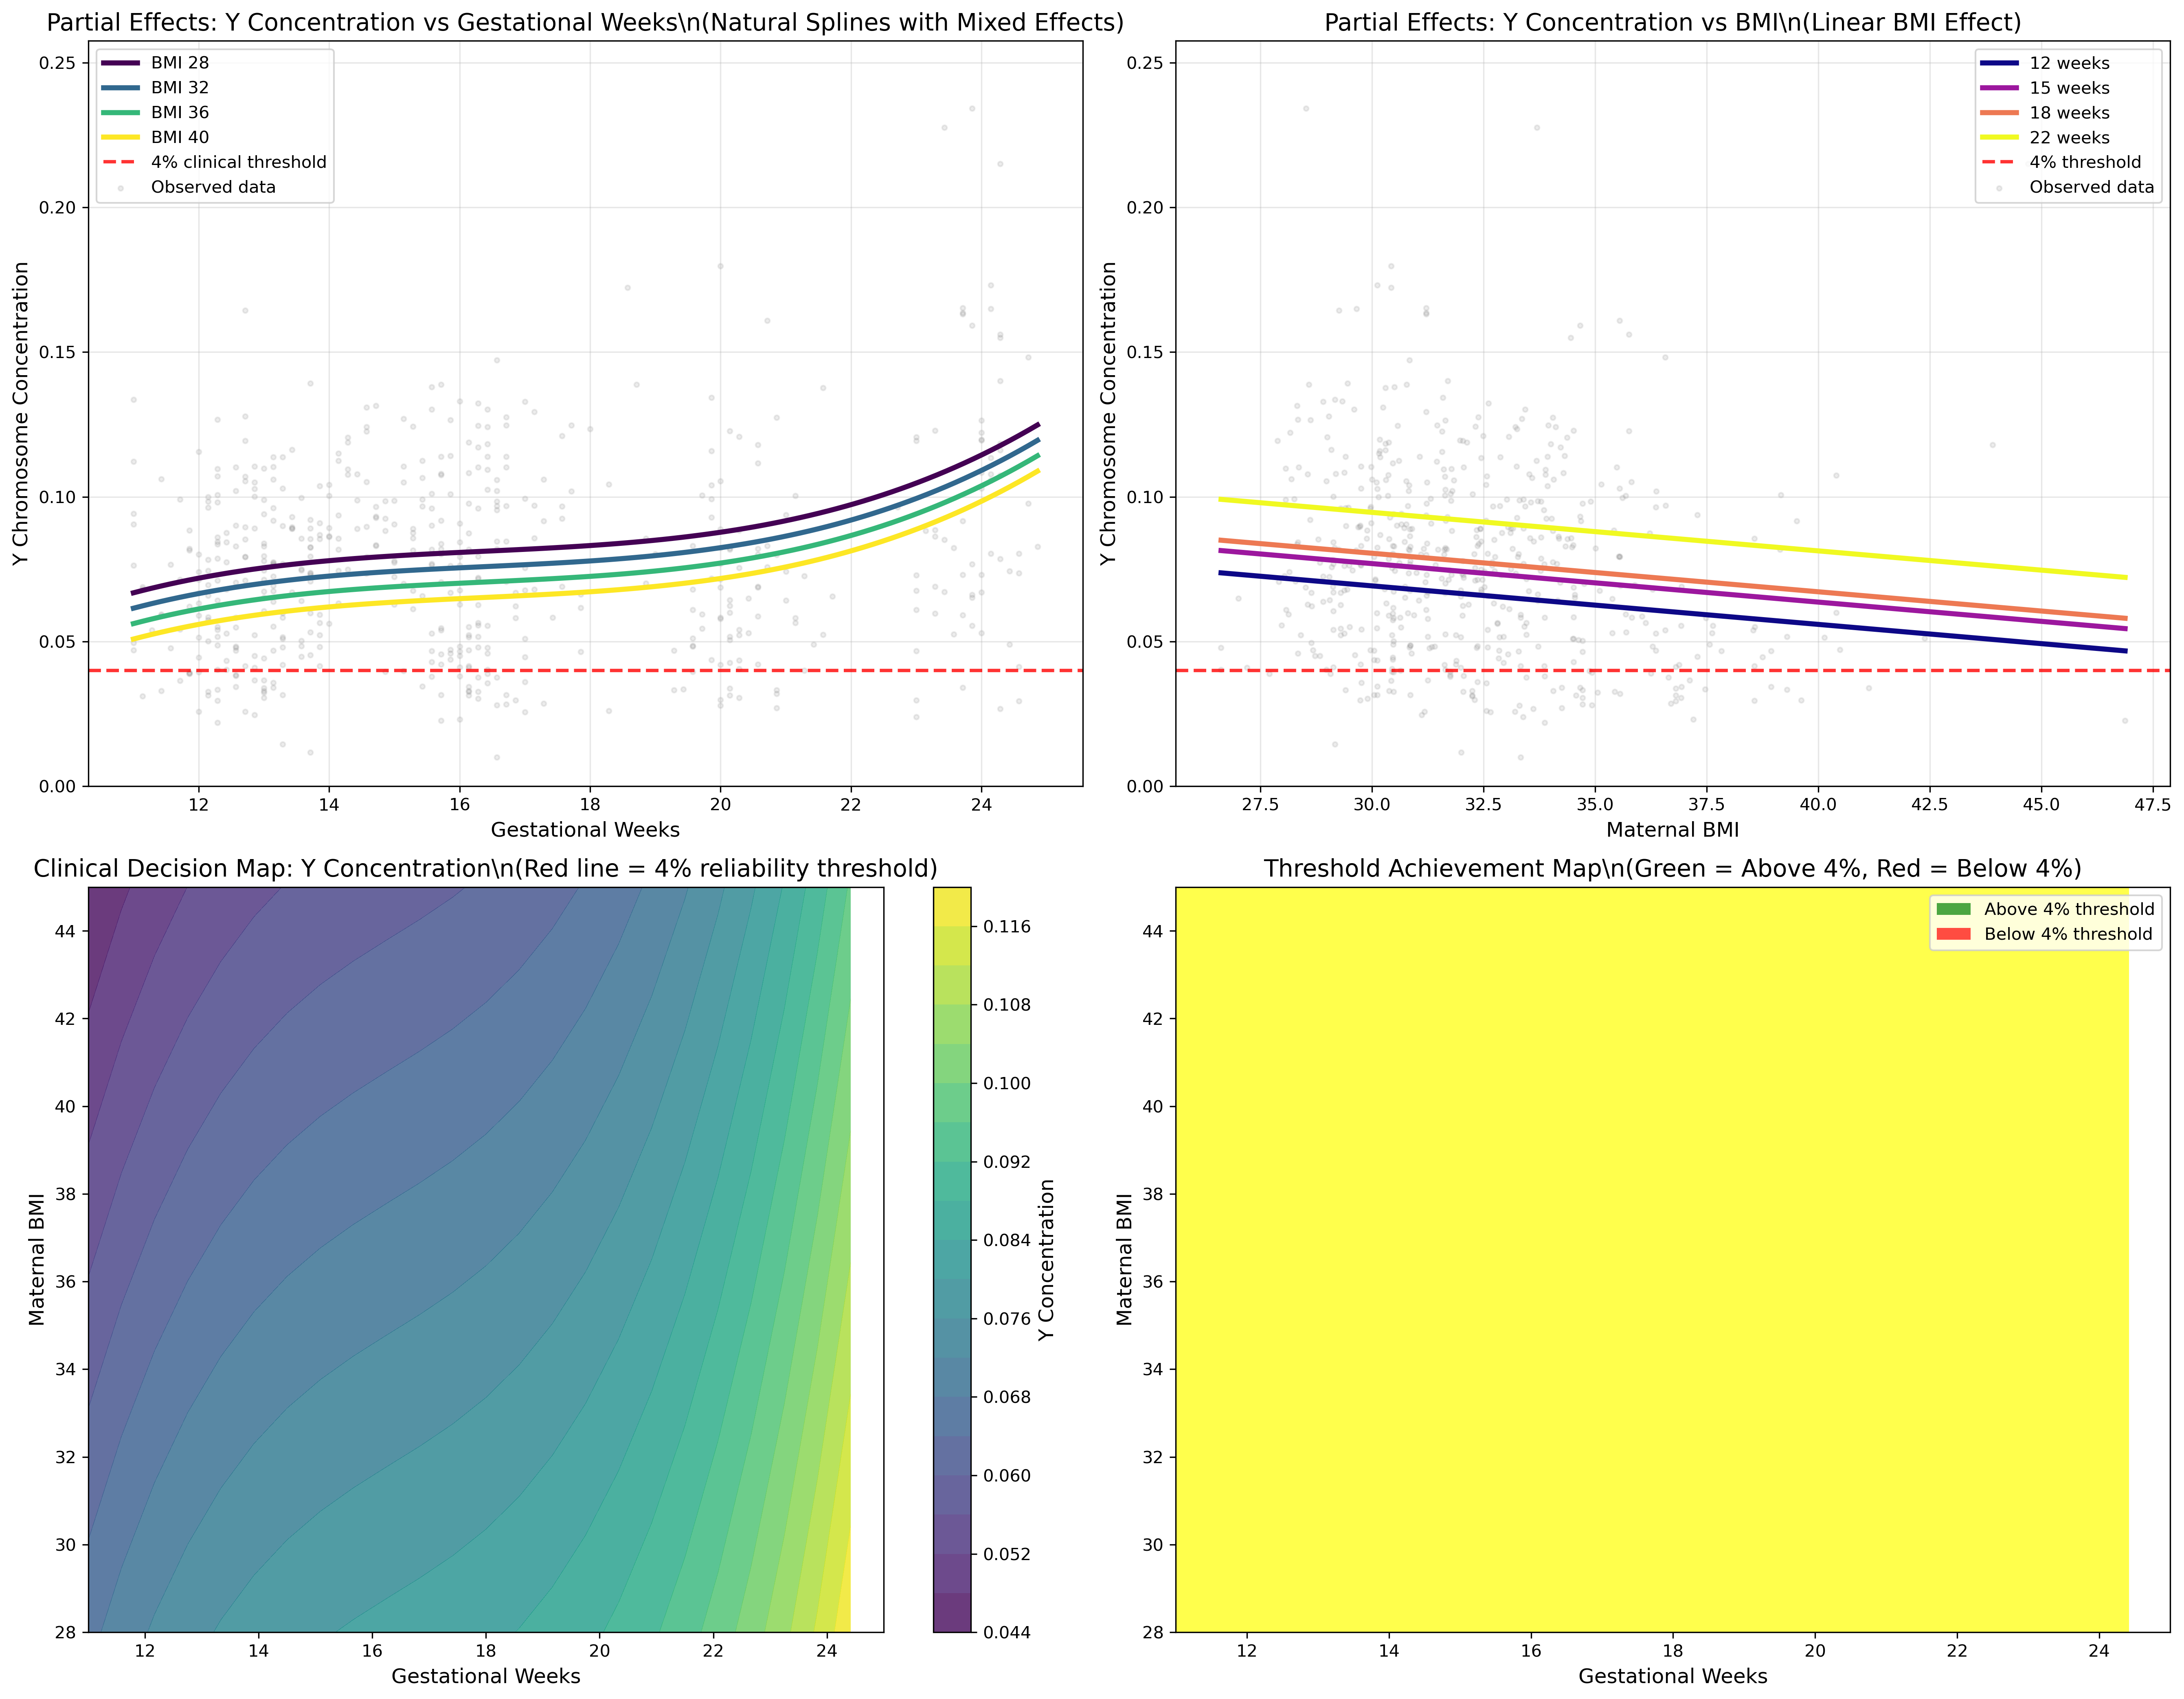
\includegraphics[width=0.8\textwidth]{output/figures/p1_comprehensive_partial_effects.png}
\caption{最终模型的部分效应与阈值地图:左/右上展示孕周与BMI的条件效应曲线,左下为连续预测等高图,右下为 $Y\ge4\%$ 区域,直观显示“孕周上升、BMI升高抑制”的结构}
\label{fig:final_partial_effects}
\end{figure}

图~\ref{fig:final_partial_effects}清晰地展示了Y染色体浓度如何随孕周和BMI变化。左上图显示,Y浓度随孕周非线性增长,早期增长较快;右上图则表明BMI对Y浓度有稳定的抑制作用。右下图的阈值地图更是直观地标示出在不同孕周和BMI组合下,Y浓度能否达到4\%的可靠性阈值,为临床决策提供了直接依据。

%(删去综合指标表以避免与模型对比表信息重叠)



\paragraph{临床二分类模型}
围绕4\%阈值的二分类Logistic建模与场景化概率表为扩展材料,此处从略,重点聚焦“Y—孕周—BMI”的关系建模与显著性验证。

\paragraph{模型对比与选择}

综合比较上述各模型,基线OLS模型虽简单但未处理非线性与聚类。仅加入样条(OLS+Splines)改善了非线性拟合($R²=0.0943, AIC=-2241.08$)但低估标准误。线性混合效应模型(Linear Mixed)处理了聚类但未捕捉非线性。最终模型(Mixed+Splines)在理论(同时处理非线性与聚类)和实证指标($AIC=-2425.94, Conditional R²=0.7476$)上均表现最优,故被选为最终模型。

针对4\%阈值的分类性能评估显示,模型具有优秀的判别能力(ROC AUC = 0.9519)。在4\%阈值下,敏感性极高(99.0\%),但特异性相对较低(45.8\%),总体准确率为92.1\%。根据Youden指数确定的最优决策阈值为5.25\%。

% (此处原有“模型的建立”占位节已上移整合,避免重复)
\subsubsection{模型的求解}
\paragraph{参数估计与设置}
连续响应的基线与样条模型使用OLS估计,并采用HC3稳健标准误进行推断,从而在存在异方差与轻度长尾时保持结论稳健。线性混合效应模型的固定效应与方差分量通过REML估计;对比含/不含样条的嵌套结构时采用极大似然(ML)评估AIC/LRT以避免REML在非嵌套固定效应比较中的偏差。样条基采用自然样条,$df=3$ 时的内部结点位于孕周分位点,确保边界外插线性与估计稳定。二分类模型采用对数似然极大化估计,并对患者聚类构造稳健簇标准误(Huber–White按个体聚类)。

\paragraph{方案与结果}
本问题的求解过程紧扣问题陈述,分为三步:分析相关特性、建立关系模型、检验显著性。
\begin{enumerate}
    \item \textbf{相关特性分析}:通过计算Pearson和Spearman相关系数(表~\ref{tab:correlation}),我们发现孕周与Y浓度呈显著正相关,而BMI与Y浓度呈显著负相关。
    \item \textbf{关系模型建立}:考虑到数据的非线性特征和重复测量结构,我们最终选定了一个混合效应模型,该模型使用自然样条来捕捉孕周的非线性影响,同时包含BMI的线性效应和代表个体差异的随机截距。其数学形式为:$Y \sim \text{bs(孕周, df=3)} + \text{BMI} + (1|\text{患者ID})$。
    \item \textbf{显著性检验}:模型的显著性通过多方面验证。首先,模型比较(表~\ref{tab:model_comparison})显示,包含样条和混合效应的模型在AIC和$R^2$等指标上均优于简单模型。其次,最终模型的参数估计(表~\ref{tab:params})显示,孕周和BMI的关键参数均具有统计显著性(p<0.05)。最后,部分效应图(图~\ref{fig:final_partial_effects})直观展示了这些显著关系。
\end{enumerate}

\paragraph{结果分析}
综合而言,我们成功地回答了问题一的三个要求:
\begin{enumerate}
    \item \textbf{相关特性}:胎儿Y染色体浓度与孕周呈非线性正相关,与BMI呈线性负相关。
    \item \textbf{关系模型}:最佳拟合模型是一个包含自然样条和随机截距的线性混合效应模型,它准确地量化了孕周和BMI对Y浓度的影响,同时考虑了个体差异。
    \item \textbf{显著性}:所有报告的关键效应均通过了统计显著性检验,证实了模型的可靠性。
\end{enumerate}
这些发现为后续问题中构建分组策略和确定最佳检测时点提供了坚实的量化基础。

\subsection{问题二的建模与求解}
\subsubsection{问题分析}
本问题旨在为男胎孕妇制定一项风险最小化的NIPT时点策略。核心任务是:根据孕妇的BMI进行合理分组,并为每组确定一个“最早安全”的抽血孕周 $w_g^{*}$,在该时点,组内孕妇的胎儿Y染色体浓度(FF)达到或超过4\%的概率至少为某一置信度 $\tau$(如90\%或95\%)。这一策略旨在通过在最优点进行检测,减少因FF浓度不足而导致的检测失败或重采血,从而最小化孕妇的潜在风险。

为实现此目标,我们将原始的重复测量数据转化为一个时间到事件(time-to-event)数据集。这里的“事件”定义为FF首次达到4\%。由于我们并非在每个时间点都观察FF,而是仅在有限的检测时点,因此首次达标的具体时间是未知的,只知道它落在一个时间区间内。这种数据结构被称为\textbf{区间删失(interval-censored)}。处理后的样本包含 $n=238$ 名孕妇,其中203名在首次检测时FF已达标(左删失),22名的达标时间位于两次检测之间(区间删失),13名在最后一次检测时仍未达标(右删失)。图~\ref{fig:p2_preprocess_time}展示了这一数据转化过程和最终的样本结构。

\begin{figure}[htbp]
\centering
\begin{subfigure}{0.48\textwidth}
  \centering
  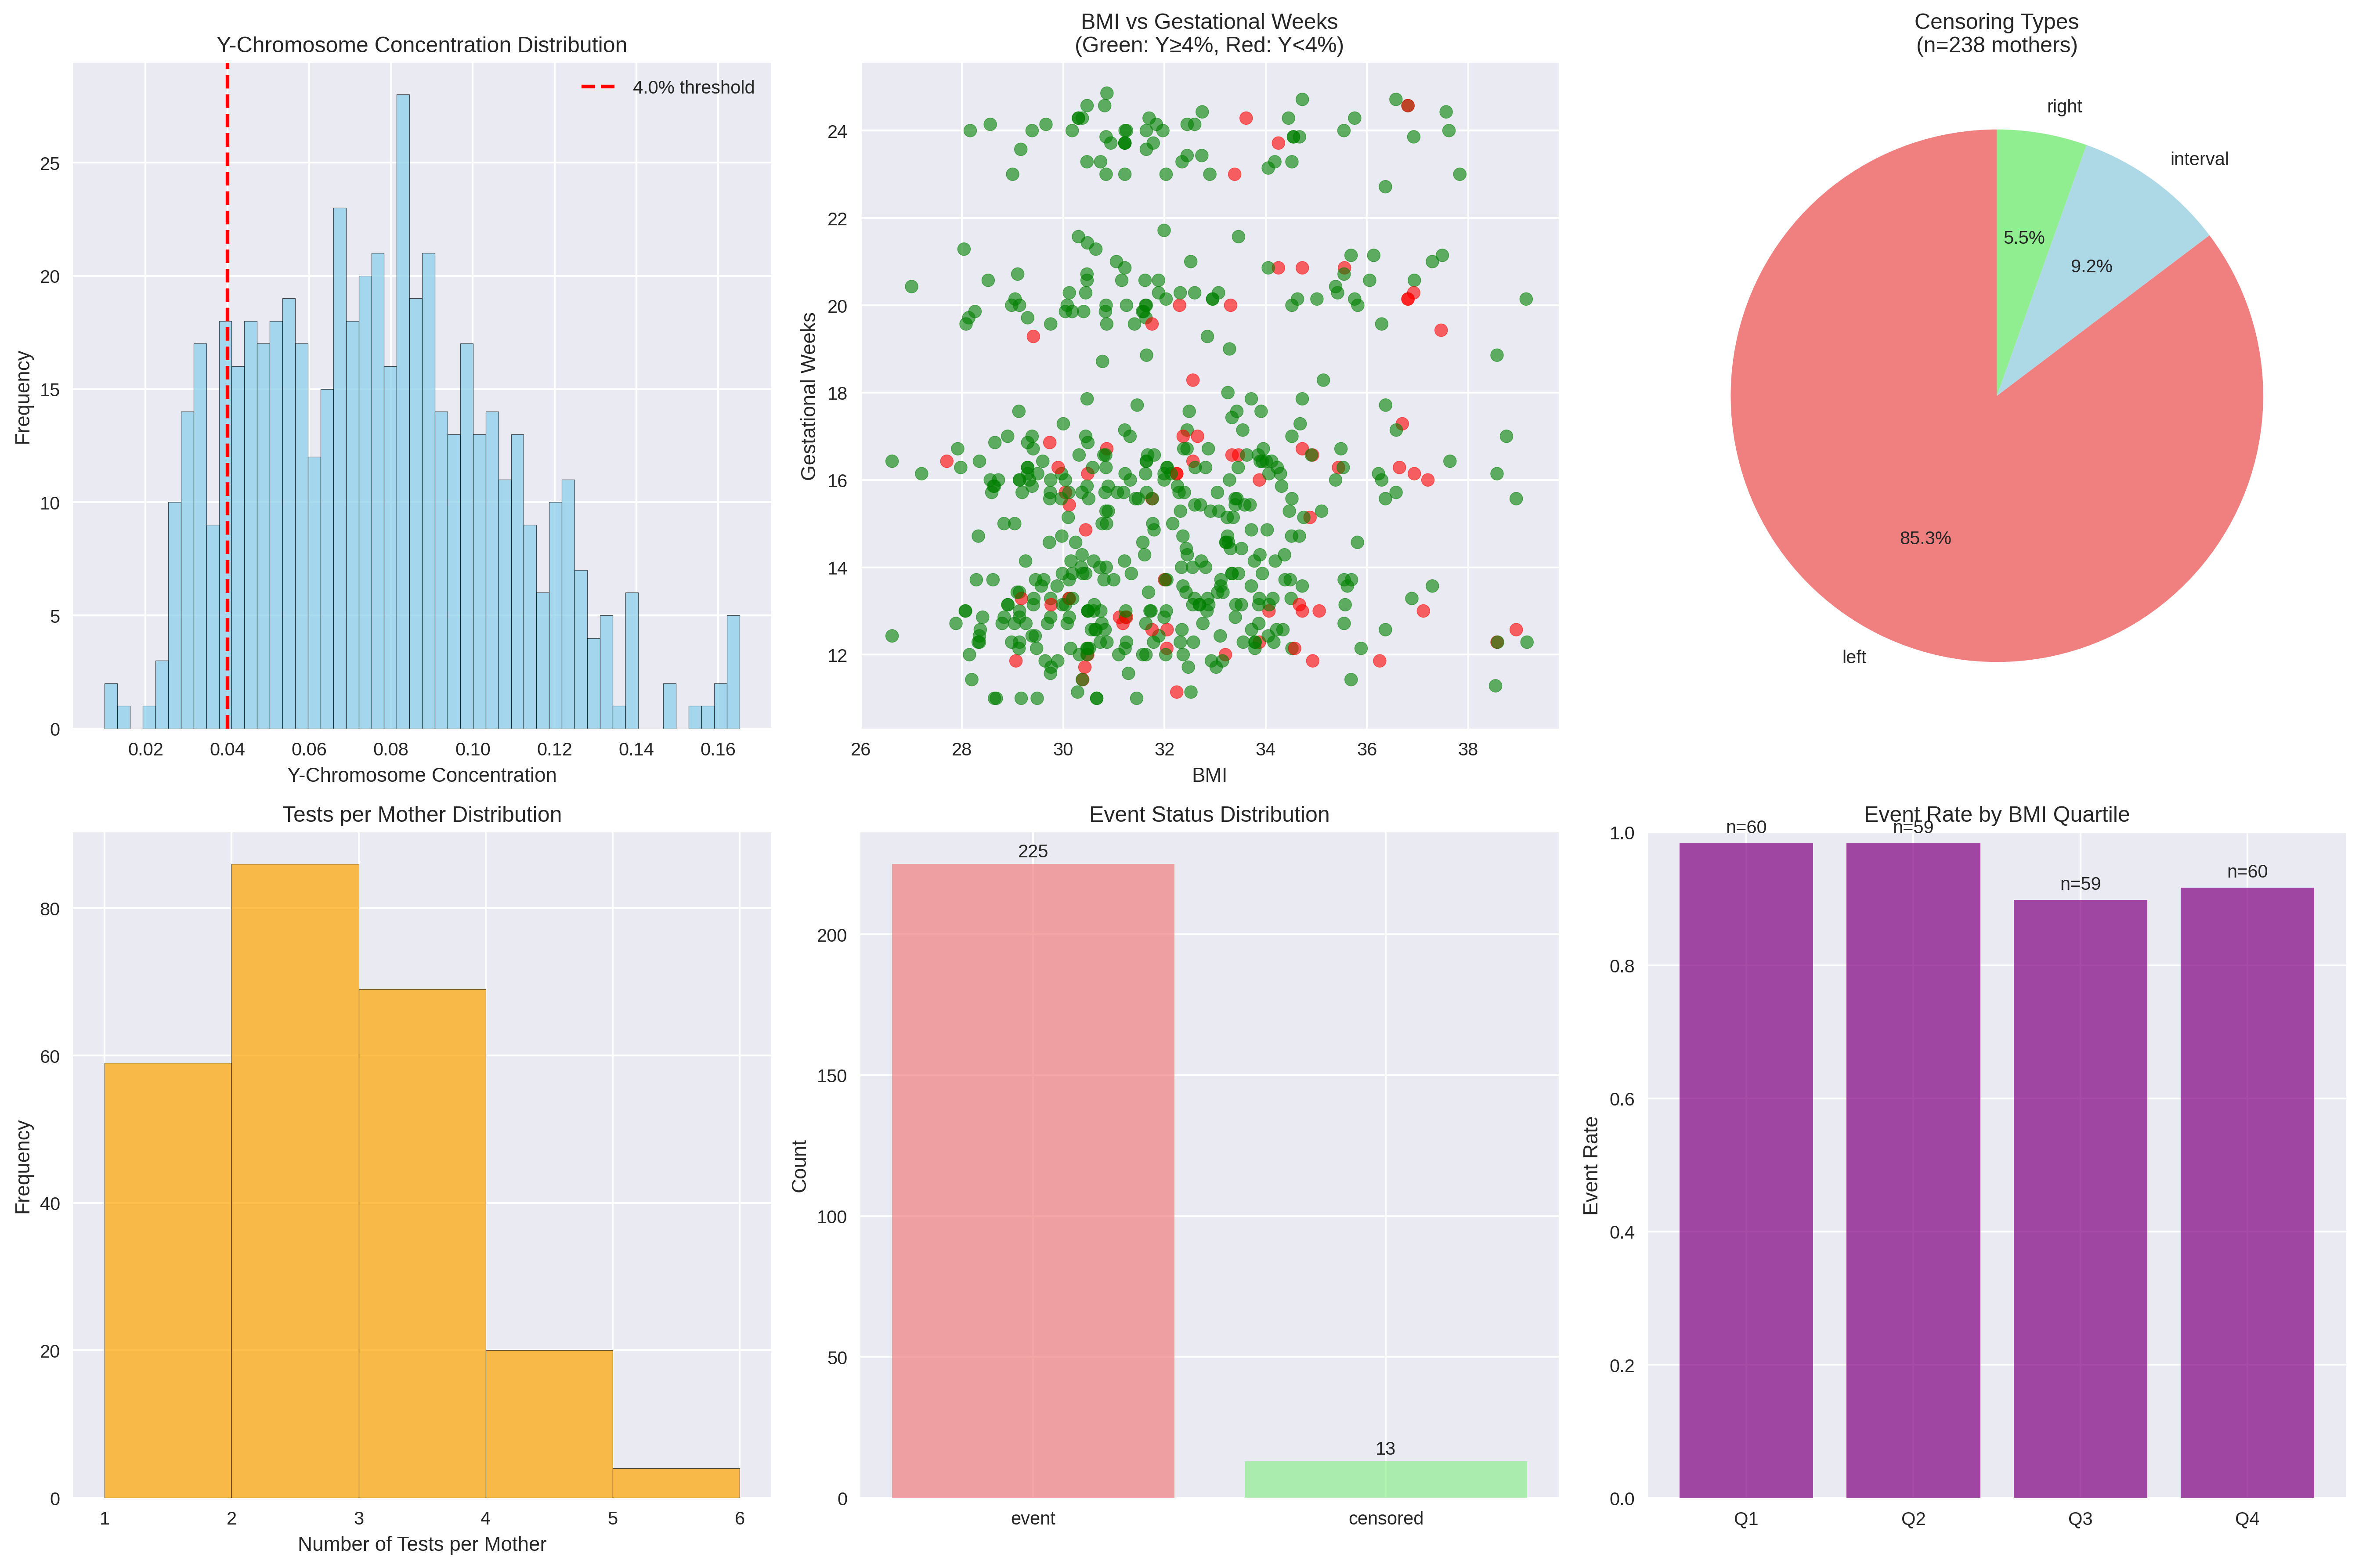
\includegraphics[width=\linewidth]{output/figures/p2_preprocessing_analysis.png}
  \caption{预处理与删失类型分布}
\end{subfigure}\hfill
\begin{subfigure}{0.48\textwidth}
  \centering
  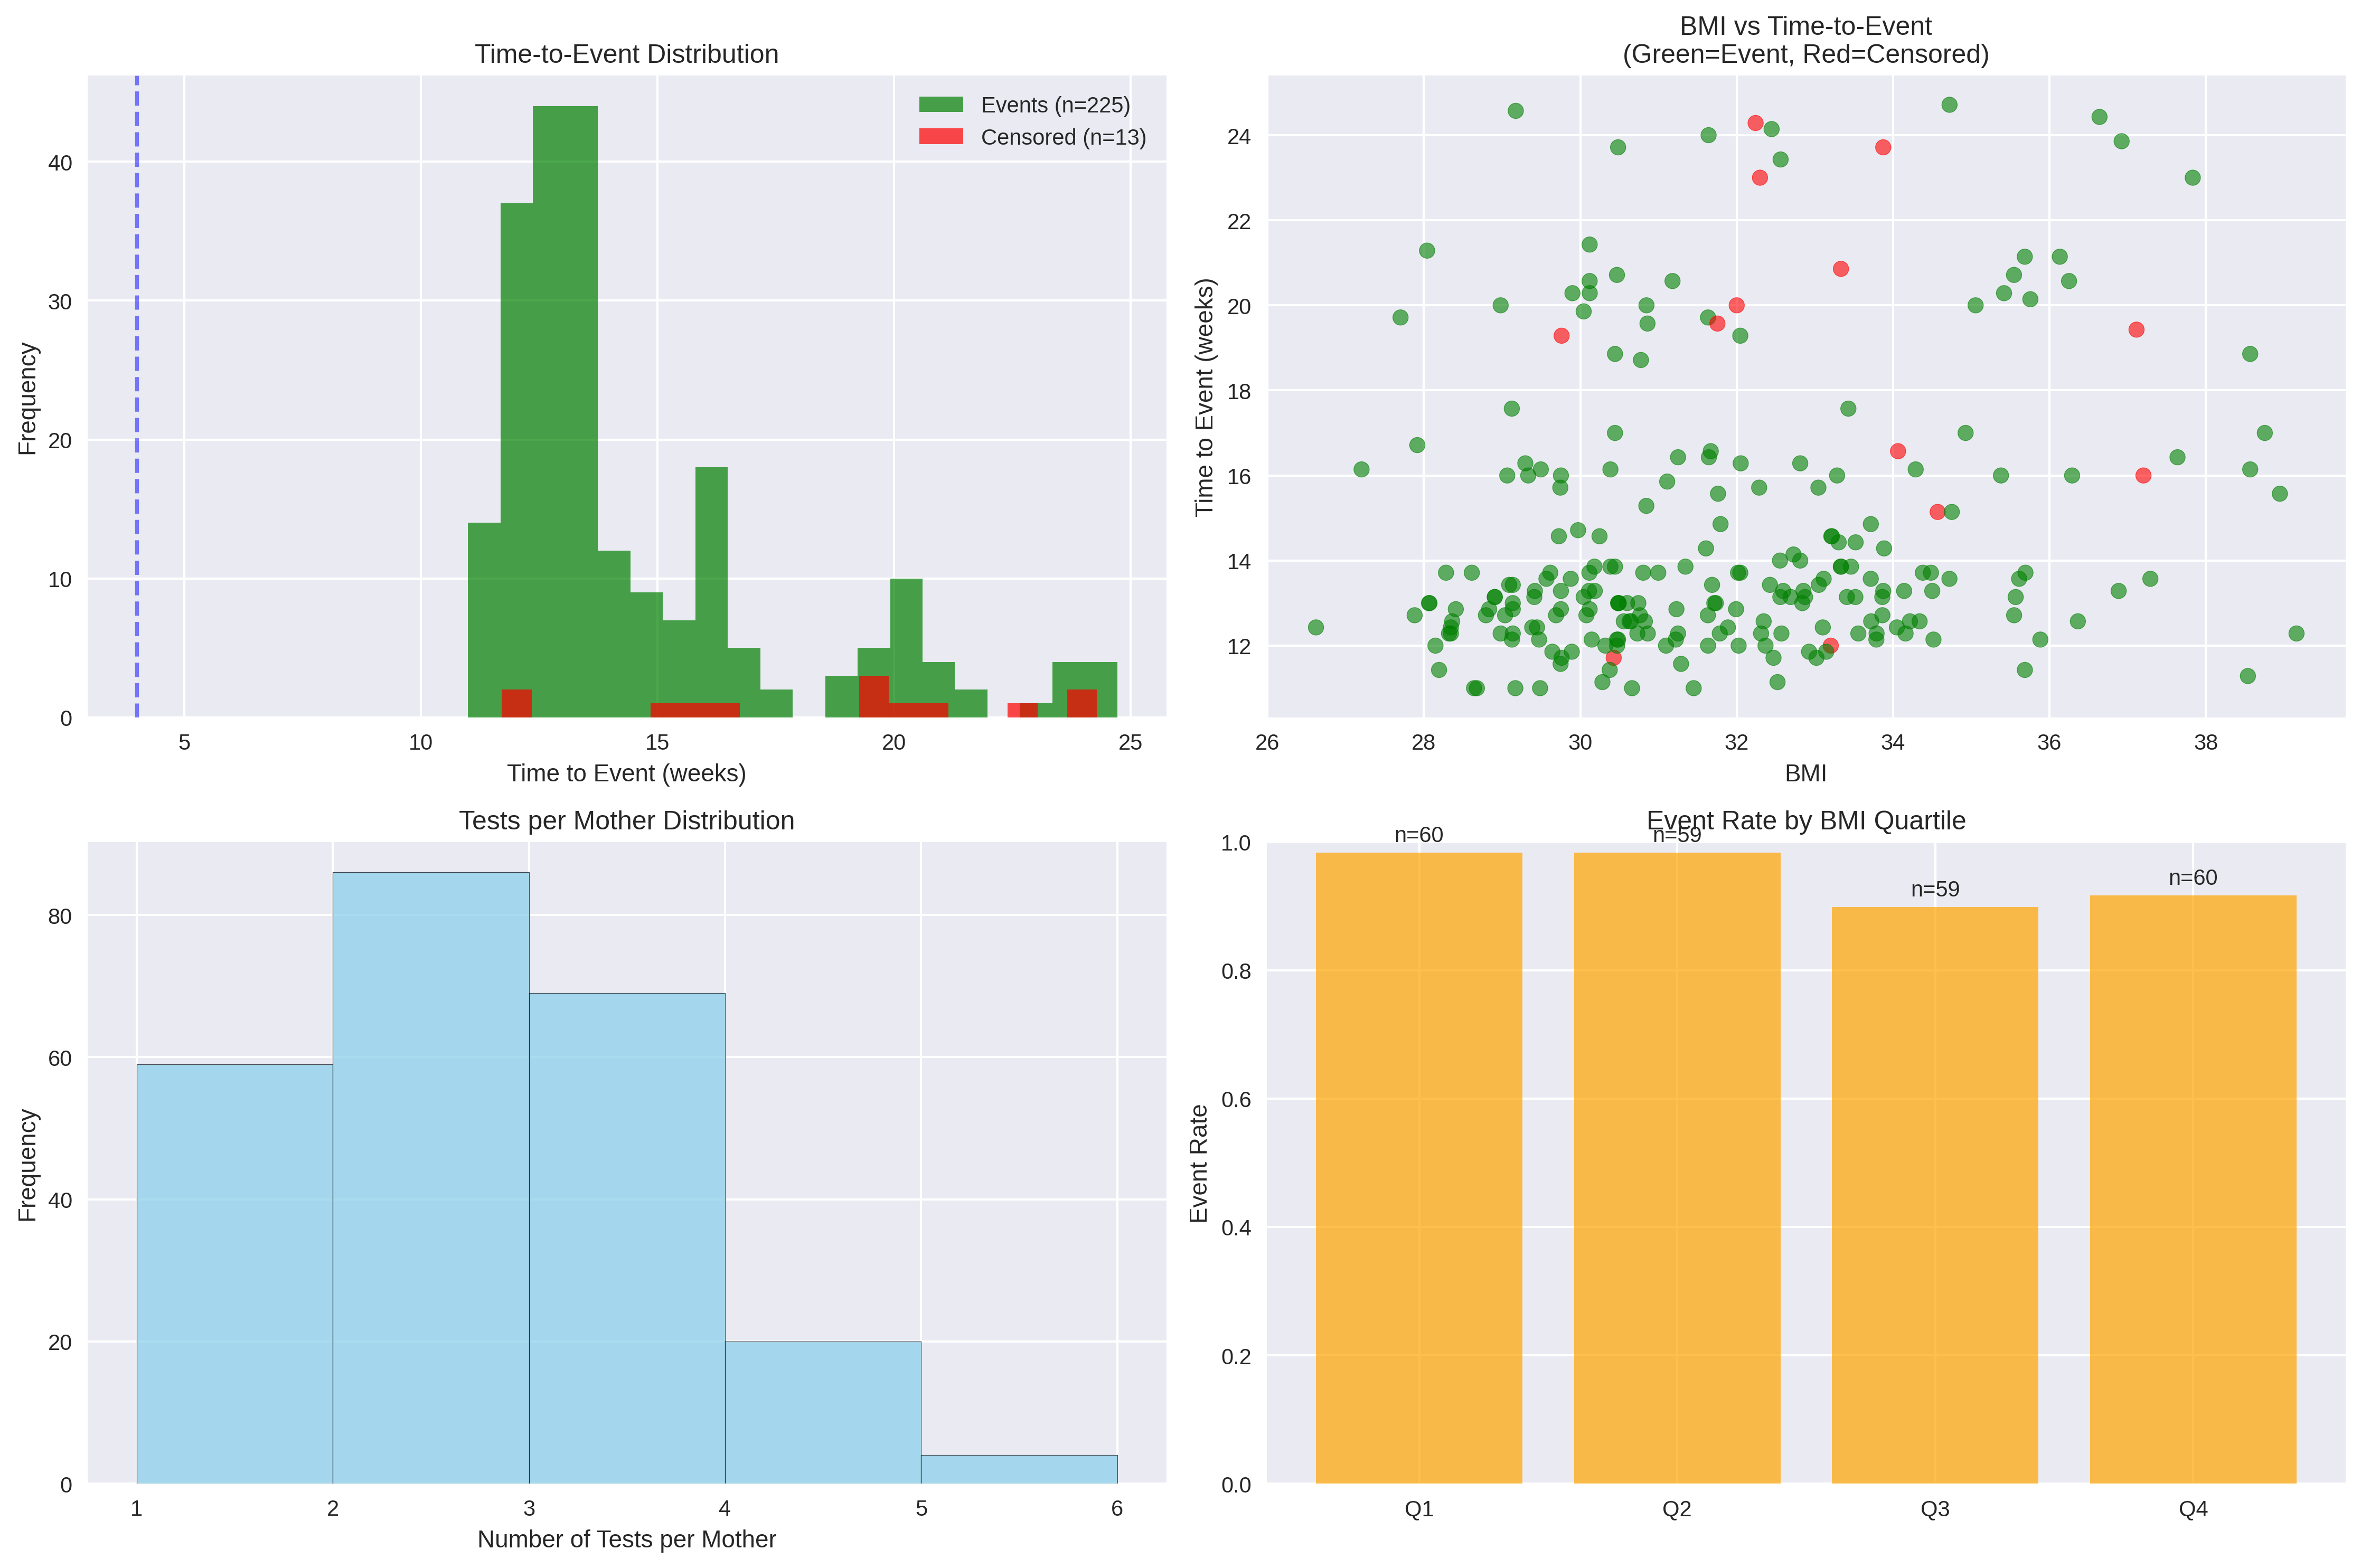
\includegraphics[width=\linewidth]{output/figures/p2_time_to_event_analysis.png}
  \caption{时间到事件构成示意}
\end{subfigure}
\caption{问题二的数据构成:区间删失(interval-censoring)框架与样本结构}
\label{fig:p2_preprocess_time}
\end{figure}
\subsubsection{模型的建立}
\paragraph{不确定性因素的定义}
检测值存在测量误差,记观测FF为 $y^{\text{obs}}=y^{\text{true}}+\epsilon$,其中 $\epsilon\sim\mathcal N(0,\sigma^2)$。误差将影响“是否达标”的判定,进而改变事件时间区间 $(L,R]$。为评估策略稳健性,我们在给定 $\sigma$ 下进行 \textbf{蒙特卡洛(Monte Carlo)} 模拟,通过对观测值添加随机扰动来重建事件区间,并重新估计模型与 $w_g^{*}$。重复此过程多次可形成 $w_g^{*}$ 的分布,从而评估其不确定性。
\paragraph{方法的引入}
主模型采用\textbf{加速失效时间(Accelerated Failure Time, AFT)}框架,这是一种生存分析模型,它直接对事件时间的对数进行建模,可以量化协变量(如BMI)如何“加速”或“减速”事件的发生。我们比较了两种基于不同分布假设的AFT模型:\emph{Weibull-AFT} 和 \emph{log-logistic AFT},并以赤池信息准则(AIC)最小者为准。令 $z(\mathrm{BMI})$ 为标准化BMI,则AFT模型写作
\[
\log T_i \,=\, \beta_0 + \beta_1\, z(\mathrm{BMI}) + \sigma\,\varepsilon_i,\qquad \varepsilon_i\sim\begin{cases}
\text{Gumbel}, & \text{Weibull-AFT}\\
\text{Logistic}, & \text{log-logistic AFT}\end{cases}
\]
相应的生存函数为 $S(t\mid x)=\Pr(T>t\mid x)$,组内(BMI组 $g$)的平均生存曲线定义为 $S_g(t)=\mathbb E_{x\in g}[S(t\mid x)]$。据此,“最早安全孕周”定义为
\[
w_g^{*}(\tau)\,=\,\inf\{t:\ 1-S_g(t)\ge \tau\},\quad \tau\in(0,1).
\]
为检验参数模型的设定合理性,我们同时拟合了\textbf{Turnbull非参数估计},这是一种处理区间删失数据的非参数方法,不依赖于特定的分布假设。通过在临床窗口(约12.0–24.7周)比较AFT与Turnbull的一致性,我们可以验证AFT模型的设定是否合理。

最后,为确定“合理”的BMI分组,我们比较了多种分组策略,包括基于临床标准的 overweight/obese 分组、三分位数分组以及由分类与回归树(CART)算法生成的分组。我们通过风险函数评估每种分组方案,该函数权衡了“时点早晚、结果稳健性、分组复杂度”三个目标。
\[
\mathcal R(G)\,=\, \sum_{g\in G} \Big( c_1\,w_g^{*}(\tau)+c_2\,\mathrm{Var}_g[w_g^{*}]\Big)\,+\,\lambda\,(|G|-1),
\]
其中 $c_1,c_2,\lambda>0$ 控制“时点早/稳健性/复杂度”的权衡。综合 CART 切分、分位法与临床分层后,选择 CART 六分组为最终策略(详见结果节)。
\subsubsection{模型的求解}
模型比较显示 Weibull-AFT 的 AIC 最小(Weibull 253.54 vs log-logistic 254.20),据此采用Weibull作为主规格。非参数 Turnbull 与 AFT 在12.0–24.7周区间的一致性优秀(MAE 0.0141、RMSE 0.0186、KS 0.0559),5-fold 交叉验证全部成功(5/5)。相关可视化见图~\ref{fig:p2_validation_survival}。

\begin{figure}[htbp]
\centering
\begin{subfigure}{0.48\textwidth}
  \centering
  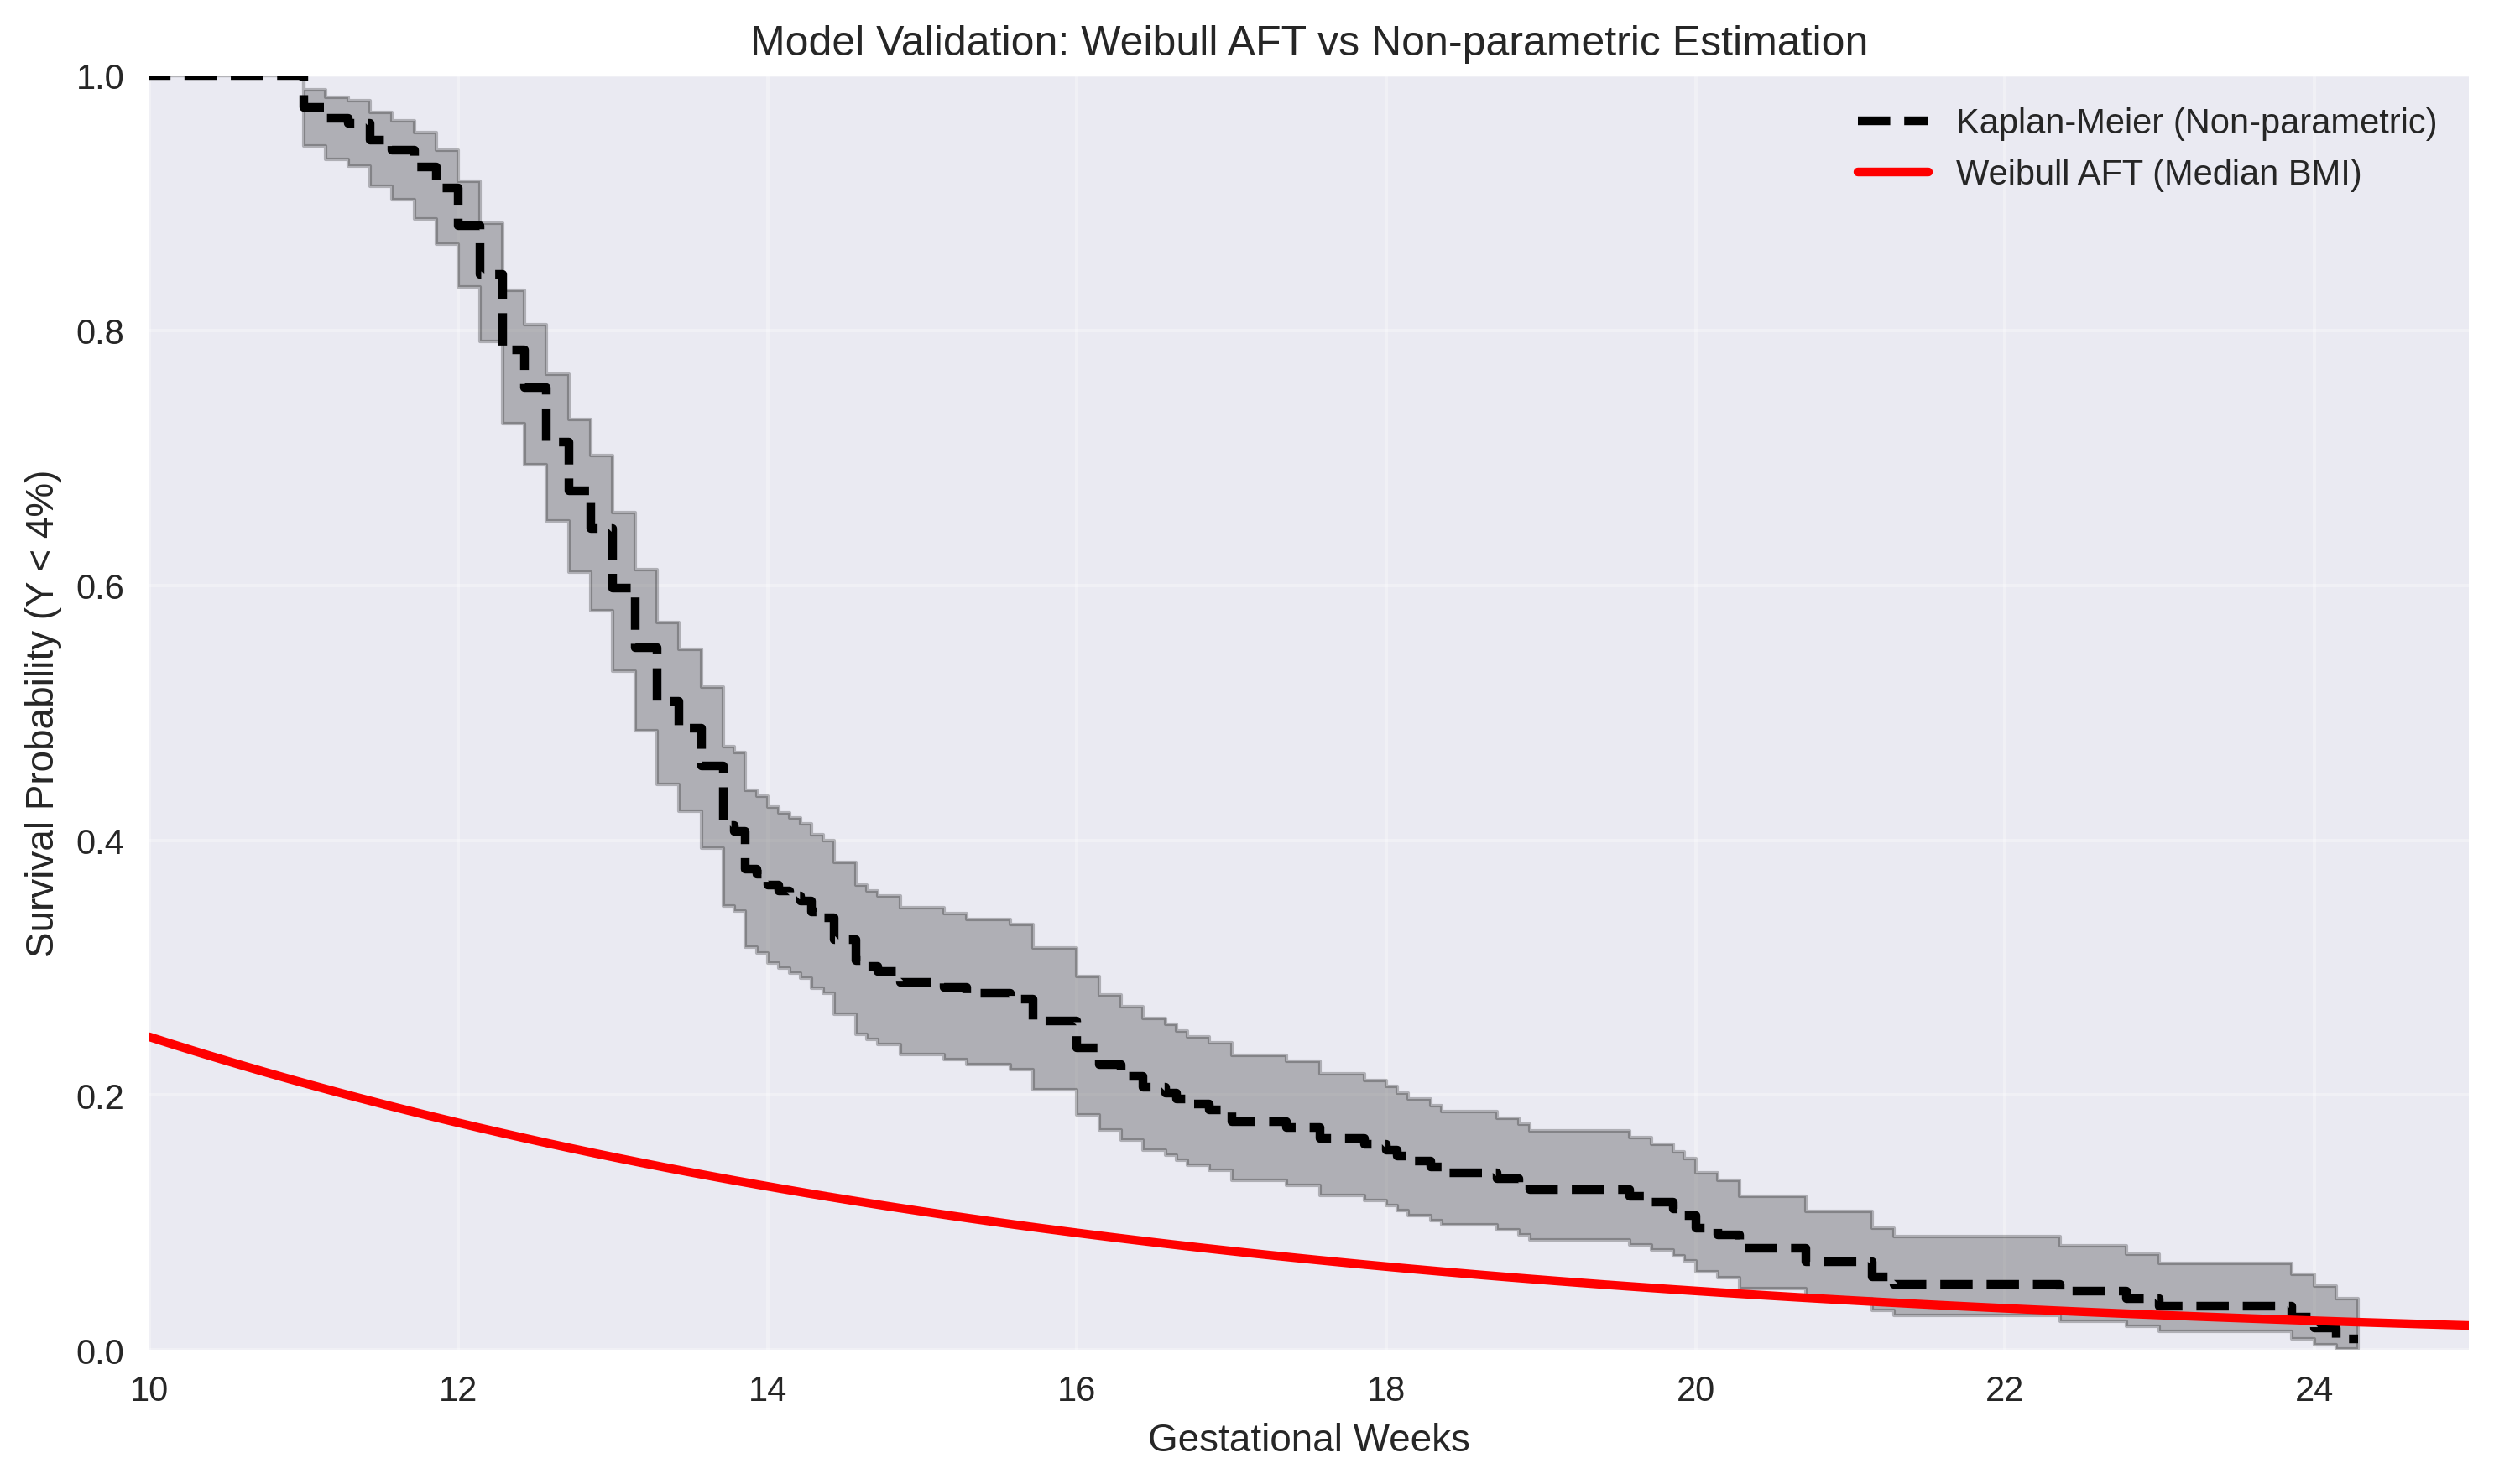
\includegraphics[width=\linewidth]{output/figures/p2_model_validation.png}
  \caption{AFT vs Turnbull 拟合一致性与CV}
\end{subfigure}\hfill
\begin{subfigure}{0.48\textwidth}
  \centering
  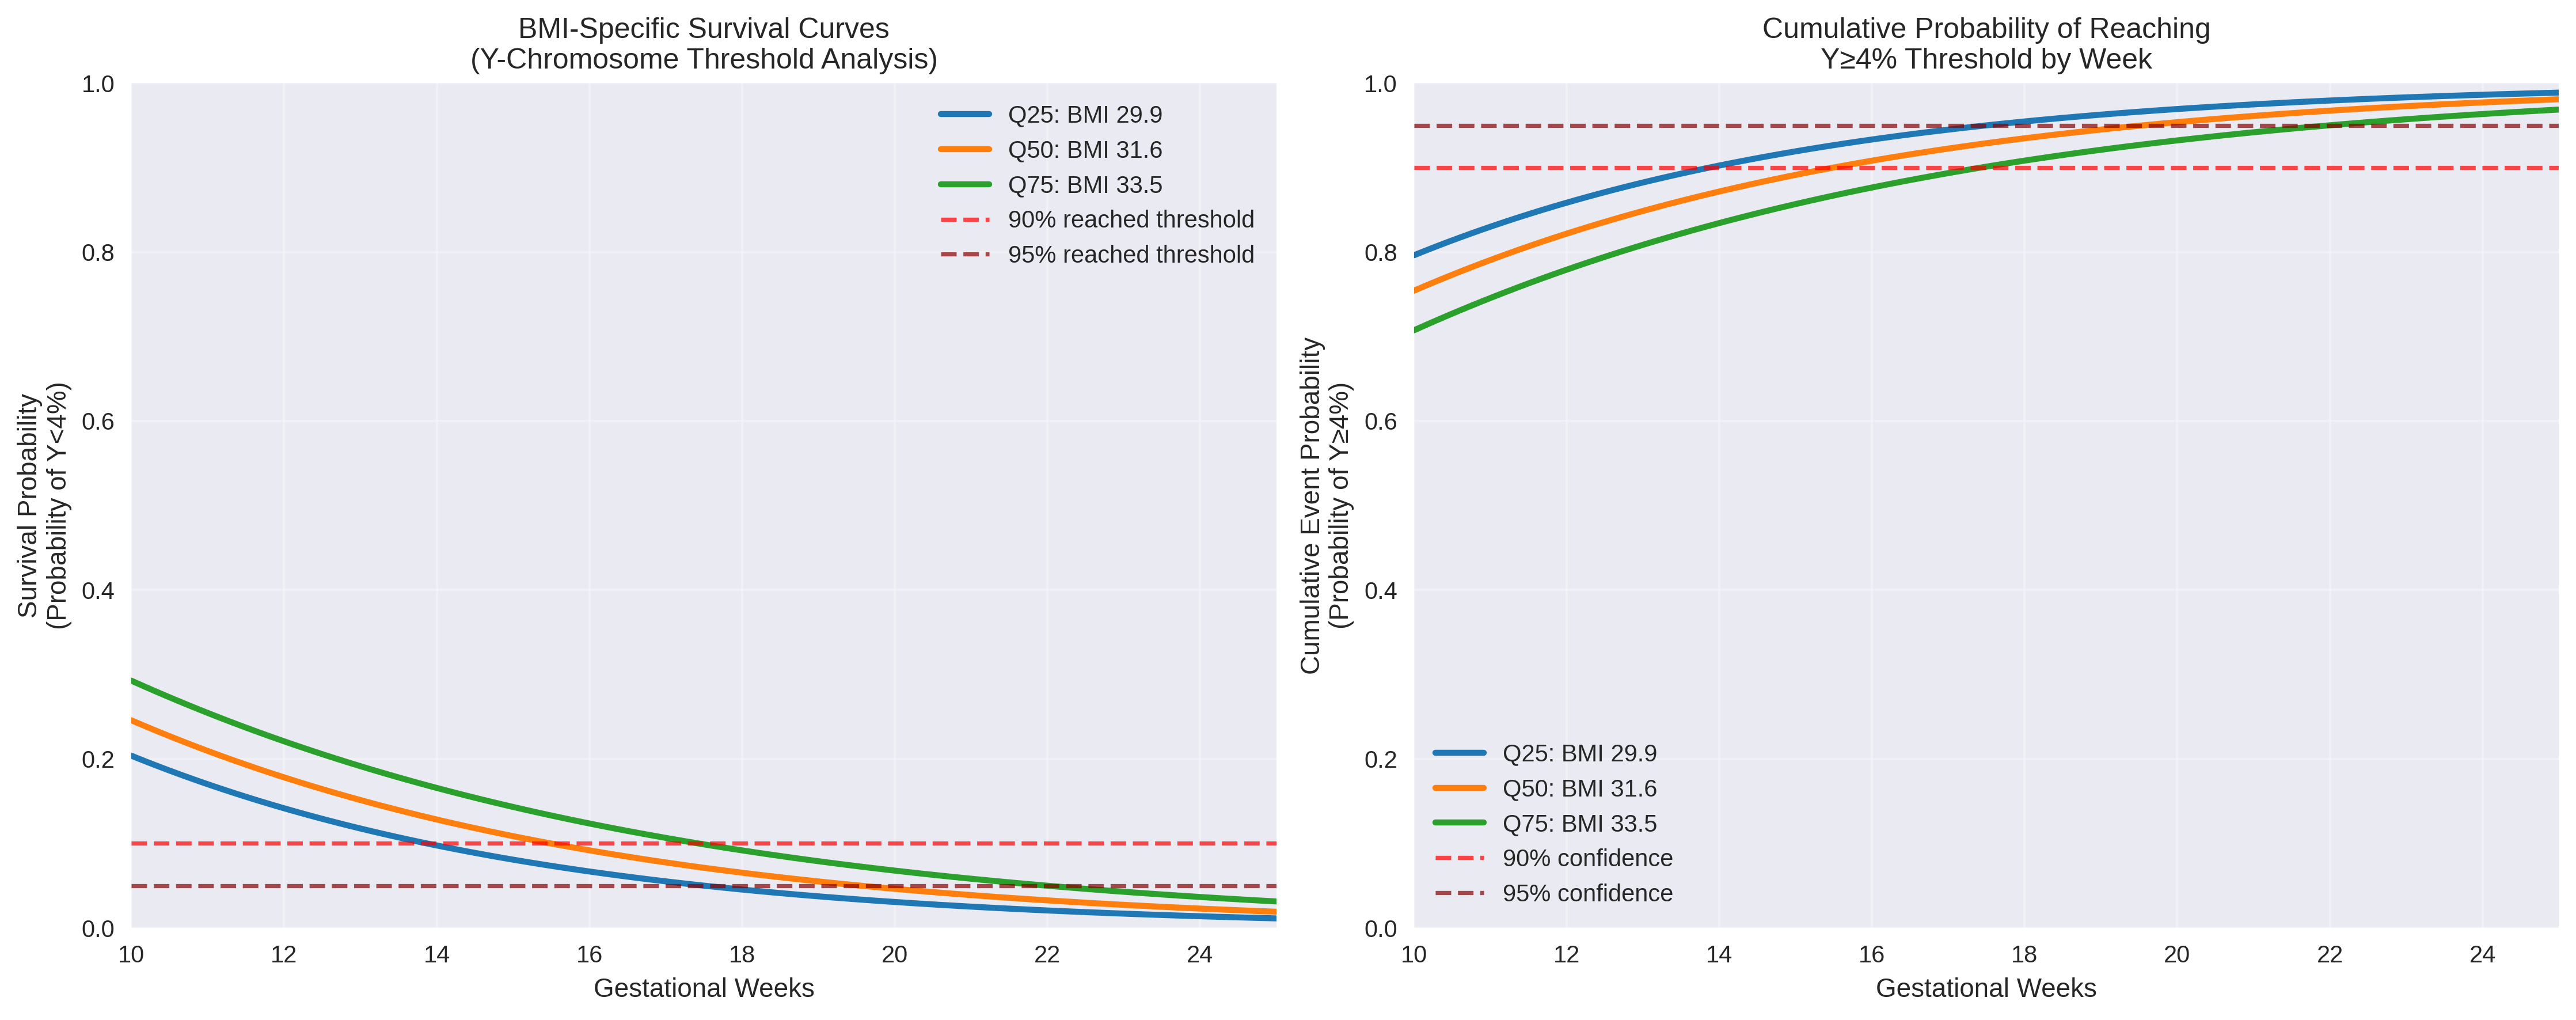
\includegraphics[width=\linewidth]{output/figures/p2_survival_curves_aft.png}
  \caption{AFT生存曲线与达标函数}
\end{subfigure}
\caption{模型充分性检验与生存曲线:AIC与非参一致性支持AFT为主结论}
\label{fig:p2_validation_survival}
\end{figure}

在分组策略选择上,我们对不同方案进行了F检验,以评估其解释方差的能力。如表~\ref{tab:p2_group_eval}所示,CART生成的六分组方案解释了最多的方差(92.5\%),表明其划分的组别内部同质性最高,组间差异最大。

\begin{table}[htbp]
\centering
\caption{分组评估(Section 5):解释方差与F统计量}
\label{tab:p2_group_eval}
\begin{tabular}{@{}lcccc@{}}
\toprule
分组策略 & 解释方差(\%) & 组间方差 & 组内方差 & F-statistic \\
\midrule
CART(6组) & 92.5 & 0.882 & 0.069 & 590.23 \\
Clinical(3组) & 77.1 & 0.734 & 0.217 & 396.74 \\
Tertile(3组) & 74.8 & 0.713 & 0.239 & 350.02 \\
\bottomrule
\end{tabular}
\end{table}

图~\ref{fig:p2_grouping}进一步从风险评分和可分性(separability)两个维度对分组方案进行了可视化比较。综合表~\ref{tab:p2_group_eval}和图~\label{fig:p2_grouping}的结果,我们最终选择\emph{CART六分组}作为最佳分组策略,因为它在最小化组内变异和最大化组间差异方面表现最优,是“合理分组”的最佳选择。各组样本规模($n=238$)为:CART\_G2=\num{58}(24.4\%)、CART\_G5=\num{46}(19.3\%)、CART\_G1=\num{38}(16.0\%)、CART\_G3=\num{35}(14.7\%)、CART\_G4=\num{31}(13.0\%)、CART\_G6=\num{30}(12.6\%)。

\begin{figure}[htbp]
\centering
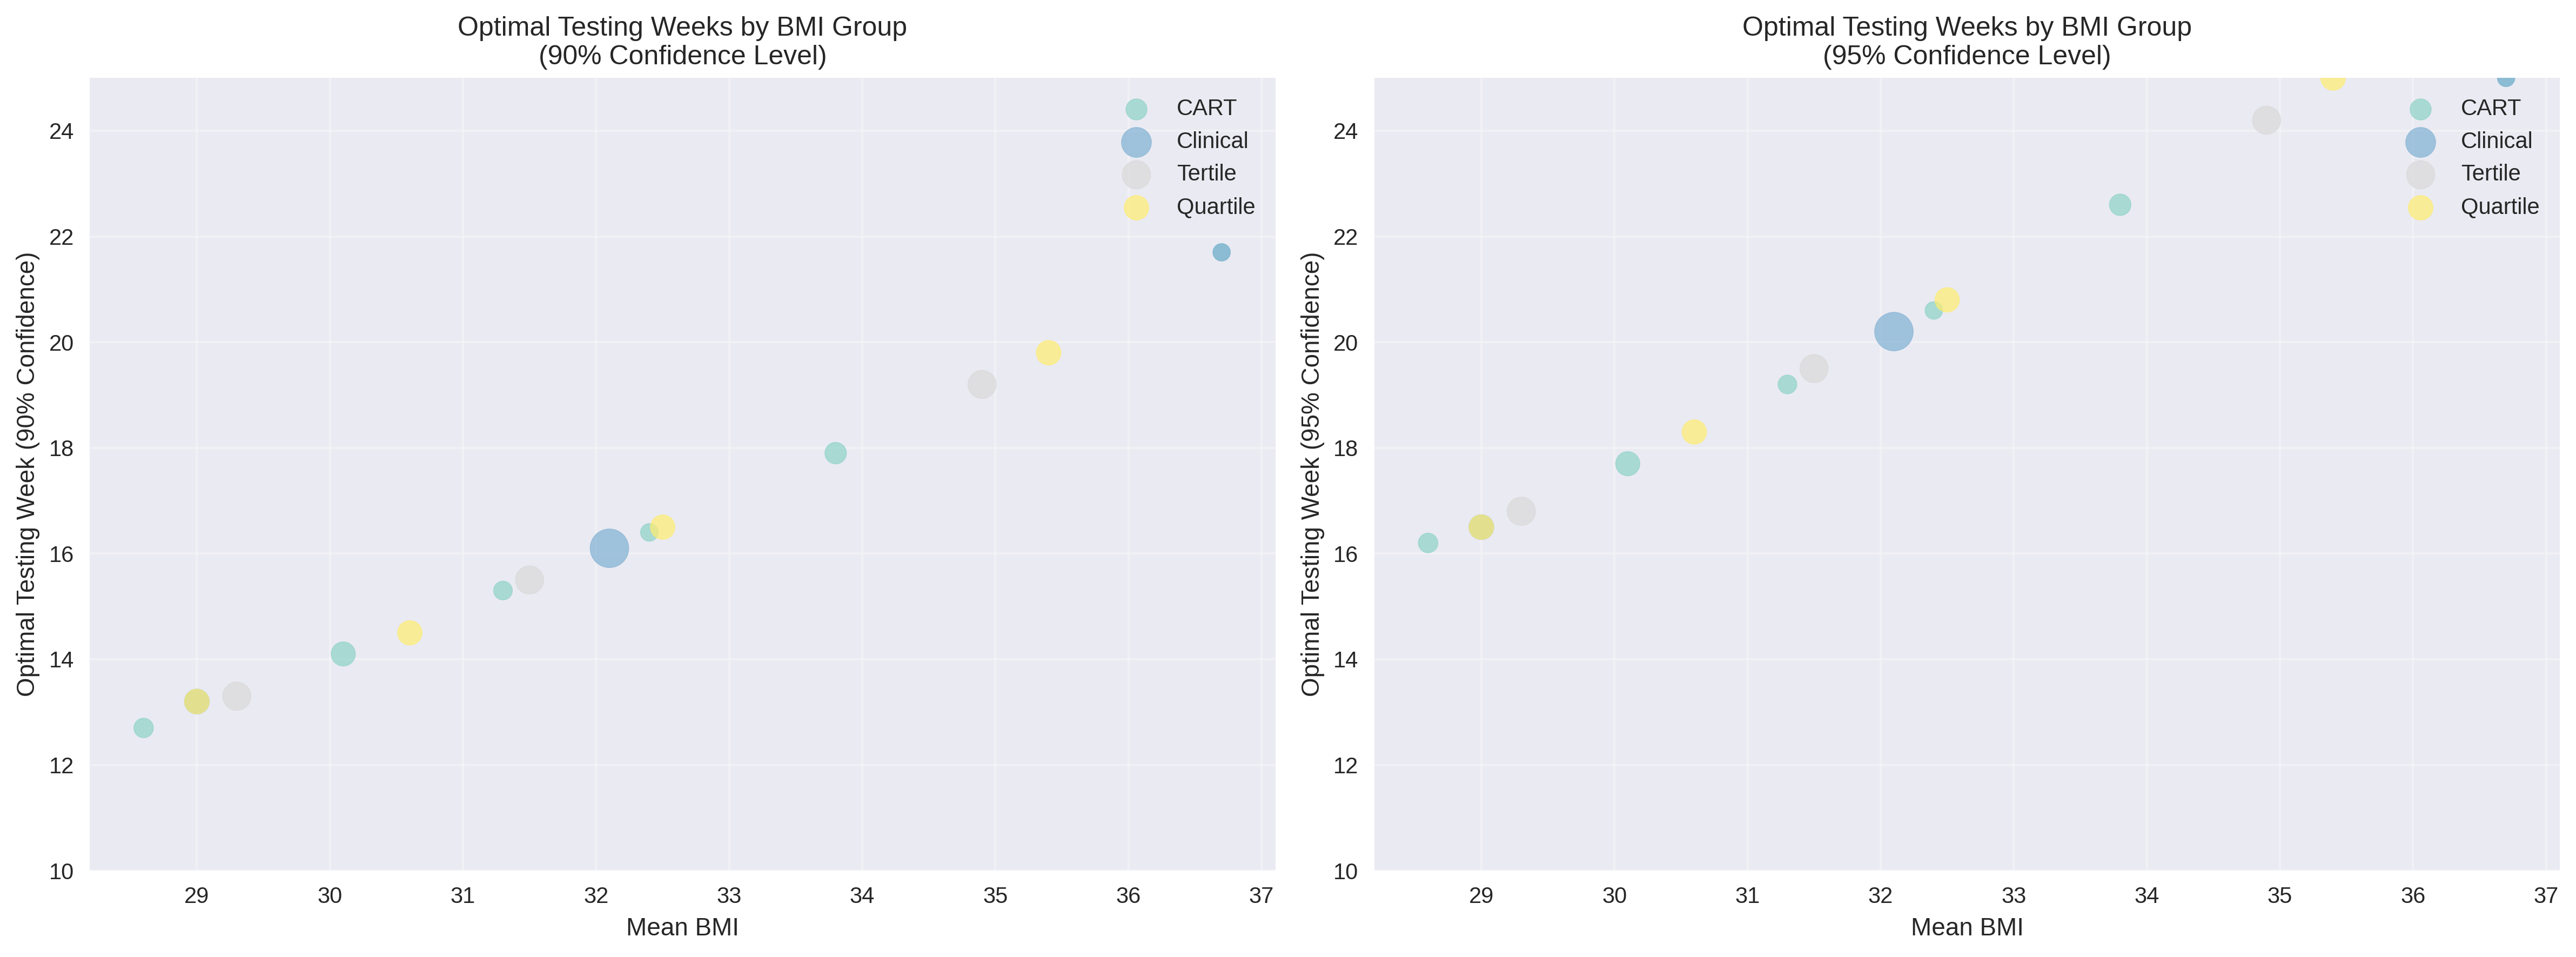
\includegraphics[width=0.7\textwidth]{output/figures/p2_bmi_groups_comparison.png}
\caption{BMI 分组方案比较(risk-score 与 separability):CART 六分组被选为最终方案}
\label{fig:p2_grouping}
\end{figure}
\subsubsection{结果与分析}
最终策略采用 \emph{CART 六分组}(CART\_G1–CART\_G6)。对 $\tau\in\{0.90,0.95\}$,我们计算各组的 $w_g^{*}(\tau)$ 并开展 Monte-Carlo($\sigma=0.002$,300次重构)稳健性评估;结果见表~\ref{tab:p2_policy}。该表是我们对问题二的核心回答,它为每个BMI分组提供了具体的最佳NIPT时点建议。
\begin{table}[htbp]
\centering
\caption{问题二策略表(CART分组):各组“最早安全孕周” $w_g^{*}(\tau)$ 及MC稳健性}
\label{tab:p2_policy}
\begin{tabular}{@{}llccc@{}}
\toprule
组别(CART) & BMI范围 & $w_{0.90}^{*}$ & $w_{0.95}^{*}$ & 说明 \\
\midrule
CART\_G1 & 26.6--29.3 & 12.9 & 16.4 & 90\%/95\%均可达标 \\
CART\_G2 & 29.4--30.7 & 14.1 & 17.9 & 均可达标,时间较G1偏晚 \\
CART\_G3 & 30.7--31.8 & 15.2 & 19.1 & BMI抬升推迟达标 \\
CART\_G4 & 31.9--32.9 & 16.4 & 20.8 & 同上 \\
CART\_G5 & 33.0--34.9 & 17.9 & 22.6 & 同上 \\
CART\_G6 & 35.1--39.2 & 21.1 & 未达到 & 95\%窗内未达(Never) \\
\bottomrule
\end{tabular}
\end{table}

从表~\ref{tab:p2_policy}中可以清晰地看到,随着BMI的升高,推荐的“最早安全孕周” $w_g^{*}$ 显著后推。例如,在90\%置信度下,最低BMI组(CART\_G1)的推荐时点为12.9周,而最高BMI组(CART\_G6)则为21.1周。在更严格的95\%置信度下,极高BMI组(CART\_G6)甚至在24.7周的临床窗口内无法达到95\%的达标概率,提示该组孕妇需要更晚的检测时点或备用筛查方案。

统计解释:(1)BMI 系数在Weibull-AFT下显著为正,表明 BMI 升高将 \emph{减速} 事件进程($T$ 变大),即推迟达标时间;(2)在 $\tau=0.90$ 下,所有 CART 组均在 12.0–24.7 周内达到阈值,而在 $\tau=0.95$ 下仅 CART\_G6 在窗口内未达(\emph{Never});(3)MC 稳健性在 $\sigma=0.002$ 下总体可接受,提示策略在现实测量扰动下具有可实施性,但对极高 BMI 组需更保守的时点或二次复检策略。

此外,低 BMI 与高 BMI 组的平均推荐时点相差约 \num{7.52} 周,与表~\ref{tab:p2_policy} 的组别结果一致,表明 BMI 升高显著推迟达标时点。
\subsubsection{小结}
本节成功地回答了问题二。我们首先将问题转化为一个区间删失的生存分析问题,并采用经过验证的Weibull-AFT模型进行建模。通过对不同分组策略的系统比较,我们确定了基于CART的六分组方案为“合理分组”的最佳选择。最终,我们给出了每个BMI分组在90\%和95\%置信度下的具体最佳NIPT时点(表~\ref{tab:p2_policy}),这一策略旨在通过在最优点进行检测来最小化孕妇的潜在风险。Monte-Carlo误差分析表明,该策略在考虑检测误差时总体上是稳健的,但对极高BMI组别,我们建议采用更保守的方案,如追加1-2周的安全缓冲,以确保检测的可靠性。

\subsection{问题三的建模与求解}
\subsubsection{问题分析}
为构建一个综合考量个体异质性、测量误差与数据删失结构的可解释性时点推荐策略,本节旨在为数据驱动的 CART-BMI 分组分别估计其``最早安全孕周'' ($w^{*}_g(\tau)$)。该时点定义为组内至少有 $\tau \in \{90\%, 95\%\}$ 比例的孕妇,其胎儿 Y 染色体浓度(FF)达到 4\% 可靠性阈值。鉴于数据集呈现出 85.0\% 的重度左删失(198/233,总检测记录数524),传统的阈值回归模型易产生偏倚。因此,我们采用区间删失(interval-censored)的生存分析框架,并以非参数 Turnbull 曲线作为基准,对参数化模型的设定充分性进行检验。此方法的核心优势在于能够充分利用不精确的事件时间信息,从而在最小化孕妇潜在风险(如不必要的重复抽血或延误诊断)的同时,提供统计上稳健的时点建议。

\subsubsection{模型的建立}
\paragraph{统计框架与目标函数} 令首次达标时间 $T$ 在区间删失框架下观测为 $T\in(L,R]$。核心模型采用 Accelerated Failure Time (AFT) 框架,并分别比较 \emph{Weibull-AFT} 与 \emph{log-logistic AFT} 两种规格;自变量包含标准化 BMI 与经特征整合后的测序/质量协变量。为处理测序质量指标间的高度相关性,我们考虑了主成分分析(PCA)进行特征整合,但最终采用方差膨胀因子(VIF)驱动的协变量选择。通过VIF控制,最终选择了6个协变量:bmi\_std, age\_std, raw\_read\_count\_std, unique\_mapped\_reads\_std, mapping\_ratio\_std, gc\_content\_std,最终VIF最大值为1.70,有效控制了多重共线性。

对 BMI 组 $g$ 的策略定义为
\[
w^{*}_g(\tau)=\inf\{t:\ 1-S_g(t)\ge \tau\},\quad \tau\in\{0.90,0.95\},
\]
其中 $S_g(t)$ 为组水平的生存函数平均。多目标风险权衡以“尽早—稳健—简洁”为原则,记(概念化)风险函数为
\[
\mathcal R(G)=\sum_{g\in G}\Big(c_1\,w^{*}_g(\tau)+c_2\,\operatorname{Var}_\text{MC}[w^{*}_g]\Big)+\lambda(|G|-1),
\]
此处的风险函数 $\mathcal R(G)$ 是一个概念化框架,用于指导我们对分组策略的评估,即在追求更早检测时点 ($w^{*}_g$ 较小) 的同时,也必须惩罚由不确定性($\operatorname{Var}_\text{MC}$ 较大)和模型复杂度($|G|$ 较大)带来的风险。在实践中,我们通过比较不同分组策略的组内方差和 F 统计量来近似此优化目标。

\paragraph{模型选择与诊断}
在包含核心变量(BMI)与扩展协变量(VIF选择后的质量指标)的模型族中,基于 AIC 的比较明确指向扩展 Weibull-AFT 模型为最优选择(AIC = 246.18,logLik = -115.09,参数8个,观测233个)。然而,需要注意的是真实事件数(区间删失事件)仅22个,事件/协变量比约3.7,明显低于常用经验规则(约10),因此统计功效有限。此外,数据结构中85.0\%的重度左删失比例极高。综合这些限制,模型在一定假定下拟合良好,但结论需谨慎解释,我们后续结合了非参数方法进行交叉验证,并执行了 Bootstrap 参数稳定性检验。相关图示见图~\ref{fig:p3_suite}。

\subsubsection{结果与分析}
\paragraph{分组对比与策略表} 依据 CART 分组(CART\_G1–G4),在 $\tau\in\{0.90,0.95\}$ 下计算各组 $w^{*}_g(\tau)$ 并给出临床建议与稳健性评估。表~\ref{tab:p3_policy_revised} 汇总了关键结果(单位:周)。可以看到,BMI 越高,推荐时点整体后移,且不确定性(MC 置信带)增宽;在 95\% 置信水平下,高 BMI 组(如 CART\_G4)可能“窗内未达”(\emph{Never}),需考虑替代流程或延后检测。

\begin{table}[htbp]
  \centering
  \caption{问题三策略表:各 CART-BMI 分组的推荐最早安全孕周 $w^{*}_g(\tau)$ 及其稳健性}
  \label{tab:p3_policy_revised}
  \begin{tabular}{@{}lccccc@{}}
    \toprule
    组别 & BMI范围 & 组内样本量 (n) & $w^{*}_{0.90}$ (周) & $w^{*}_{0.95}$ (周) & 95\% MC IQR ($w^{*}_{0.90}$) \\
    \midrule
    CART\_G1 & 26.6--29.4 & 39 & 12.50 & 15.70 & [11.2, 13.7] \\
    CART\_G2 & 29.4--31.3 & 73 & 15.00 & 18.80 & [14.0, 15.9] \\
    CART\_G3 & 31.3--33.3 & 57 & 15.00 & 19.20 & [13.8, 16.1] \\
    CART\_G4 & 33.3--39.2 & 64 & 20.70 & 未在观测窗口内达到 & [18.6, 22.8] \\
    \bottomrule
  \end{tabular}
\end{table}

组间对比(group contrasts)显示,在 90\% 置信水平下,CART\_G4 相较 CART\_G2 晚约 \num{5.7} 周、相较 CART\_G1 晚约 \num{8.2} 周;在 95\% 置信水平下,部分高 BMI 组呈"\textit{inf}"现象,提示严格置信标准下需采用延后检测或二次复检策略。

\paragraph{AFT参数解释与时间比} 扩展Weibull-AFT模型的时间比(time ratio/acceleration factor)解释如下:bmi\_std的Bootstrap估计为1.160(95\% CI: 1.066–1.328),mapping\_ratio\_std也显著大于1。时间比>1表示达标时间延长(即更晚达标)。具体而言,BMI标准化每增加1个单位,预期达标时间延长约16.0\%;测序比对率的提升反而与达标时间延迟相关,可能反映高BMI个体的测序复杂性。Monte-Carlo模拟(300次运行,收敛率100\%)与Bootstrap分析(50次重抽样)均支持这一结论的稳健性。

\paragraph{稳健性与不确定性} MC 评估表明:在 $\tau=0.90$ 下,CART\_G1/G2/G3 的置信带宽约为 \num{2.43}/\num{1.97}/\num{2.27} 周,较为集中;而高 BMI 组(CART\_G4)带宽增至 \num{4.24} 周,不确定性显著上升。结合模型诊断"重度左删失"的提示,我们建议对高 BMI 组在 0.90 方案上增加 1–2 周的安全缓冲,或采用 0.95 的更严格阈值并配合备用流程。

\begin{figure}[htbp]
\centering
\begin{subfigure}{0.48\textwidth}
  \centering
  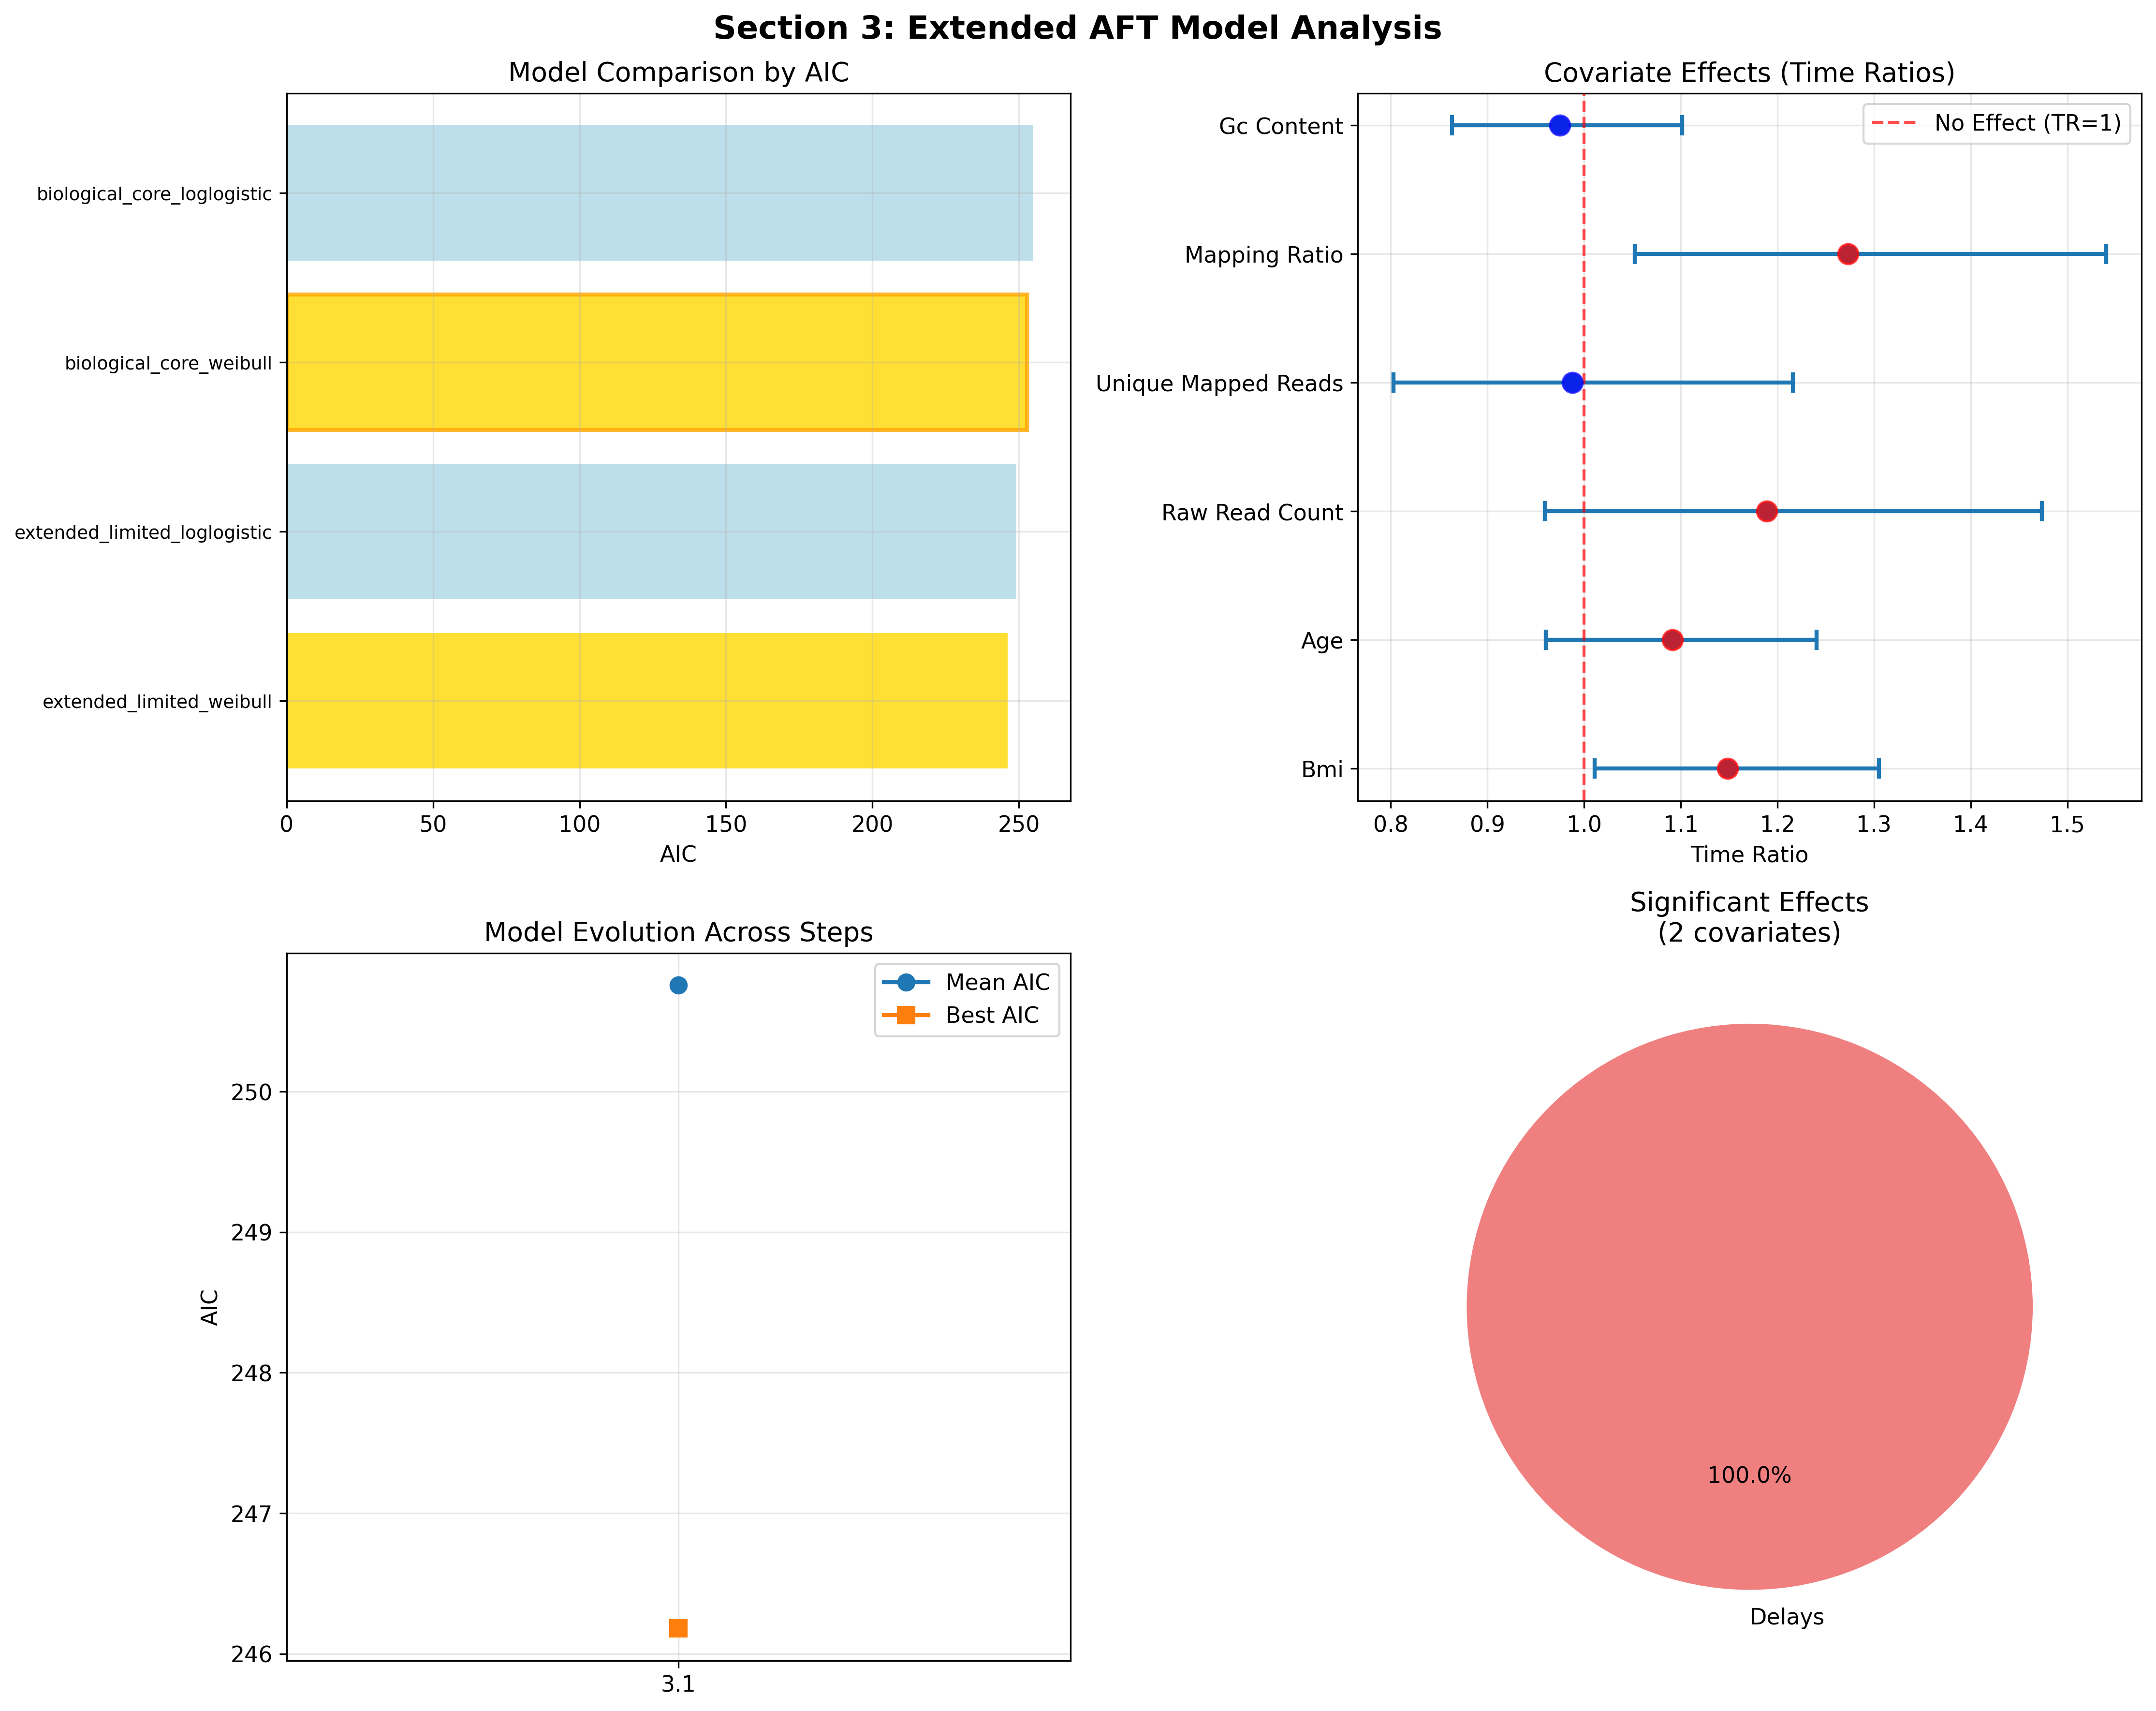
\includegraphics[width=\linewidth]{output/figures/p3_section3_aft_model_analysis.png}
  \caption{AFT 模型比较(AIC 与拟合)}
\end{subfigure}\hfill
\begin{subfigure}{0.48\textwidth}
  \centering
  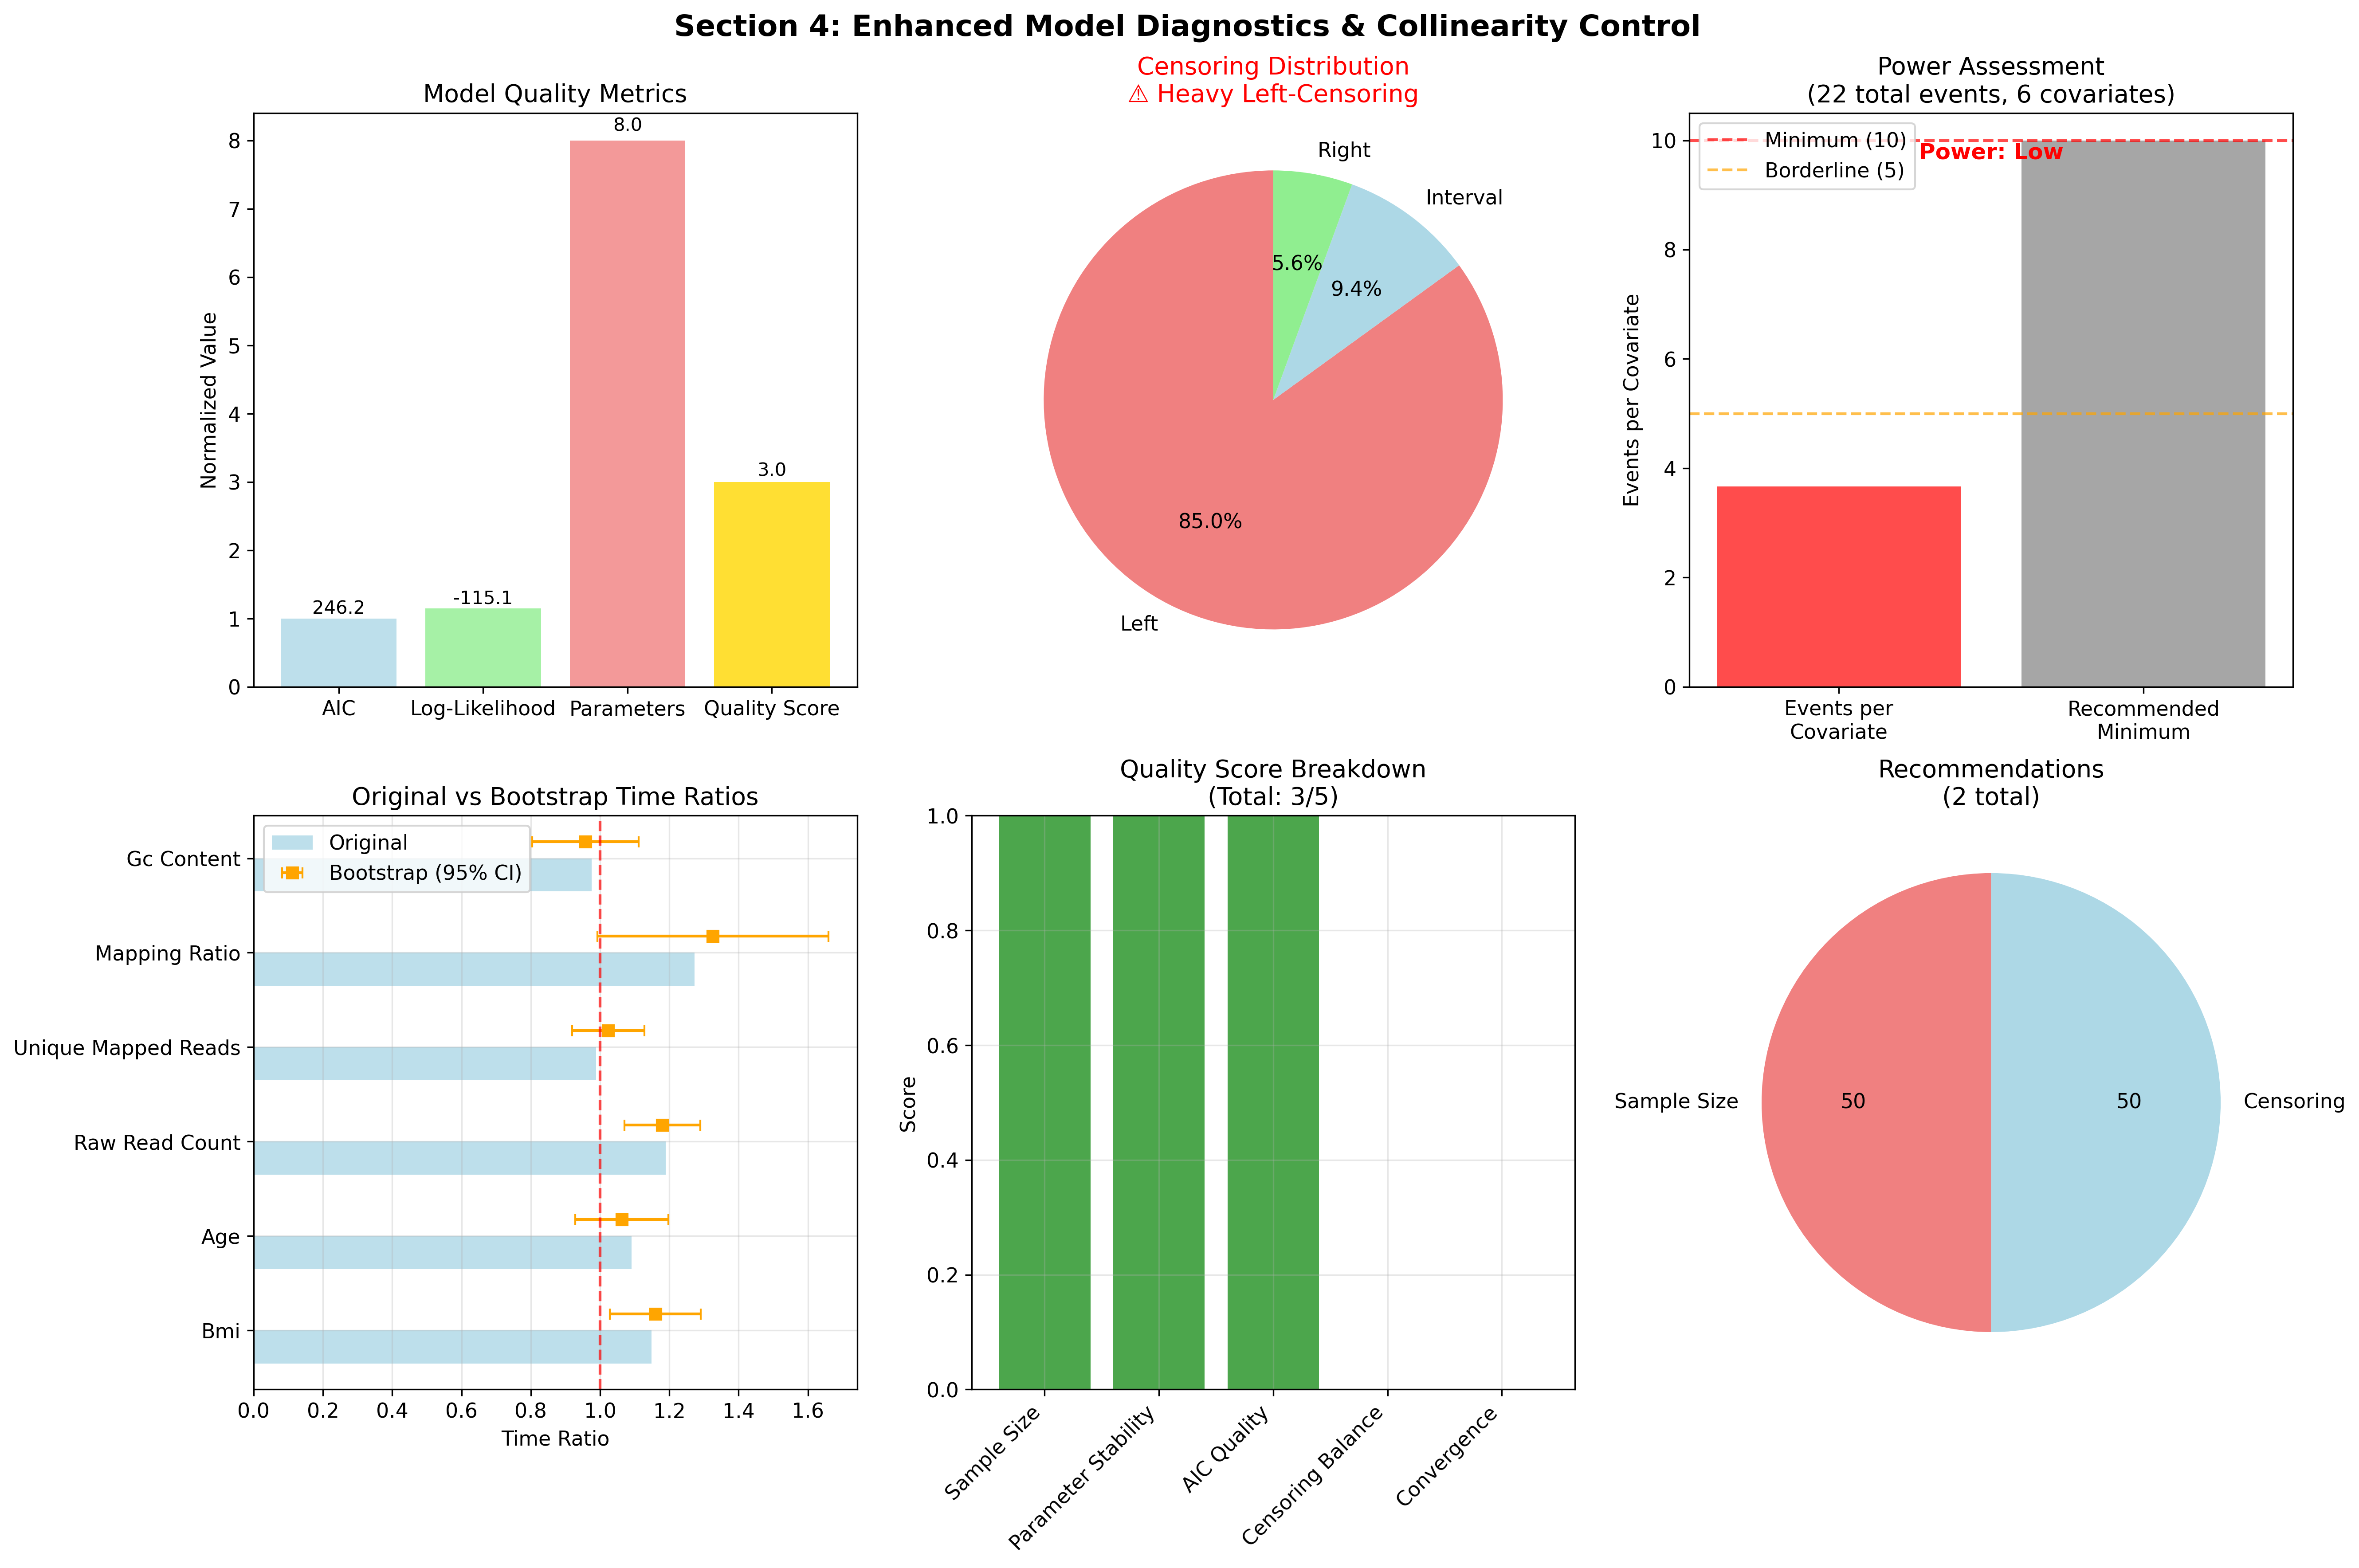
\includegraphics[width=\linewidth]{output/figures/p3_section4_model_diagnostics.png}
  \caption{删失结构与诊断}
\end{subfigure}\\[4pt]
\begin{subfigure}{0.48\textwidth}
  \centering
  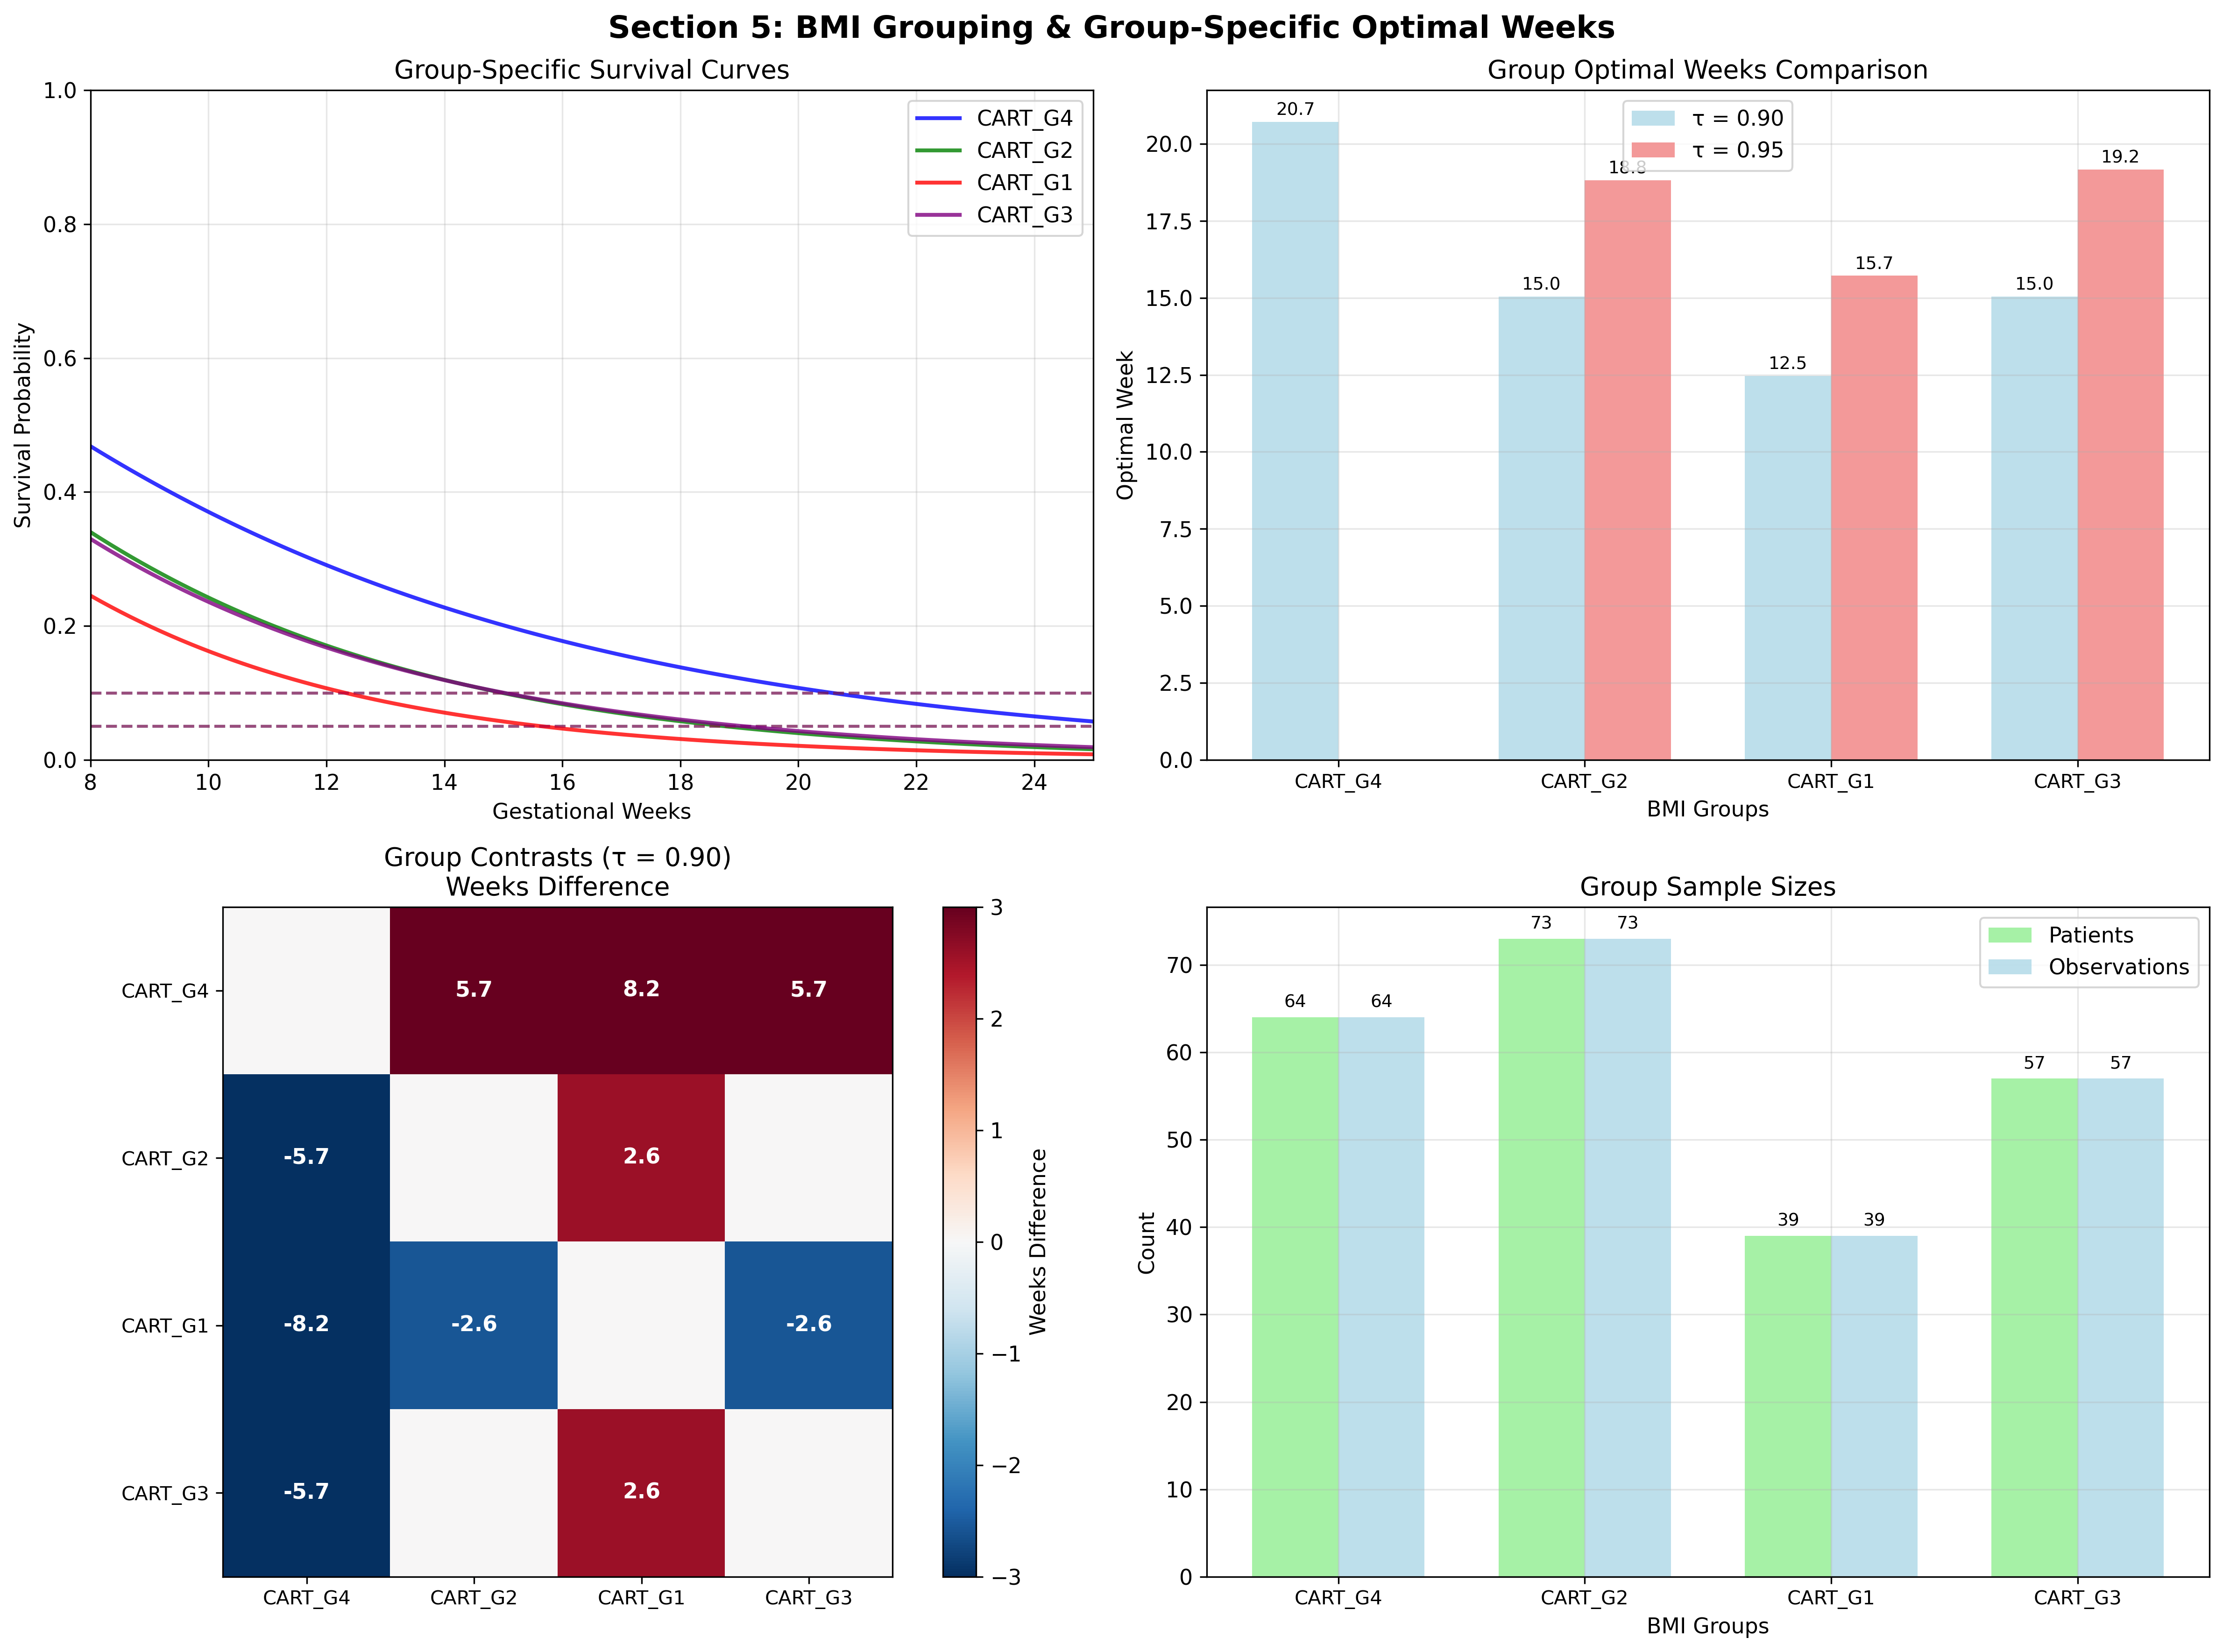
\includegraphics[width=\linewidth]{output/figures/p3_section5_group_analysis.png}
  \caption{CART 分组效应}
\end{subfigure}\hfill
\begin{subfigure}{0.48\textwidth}
  \centering
  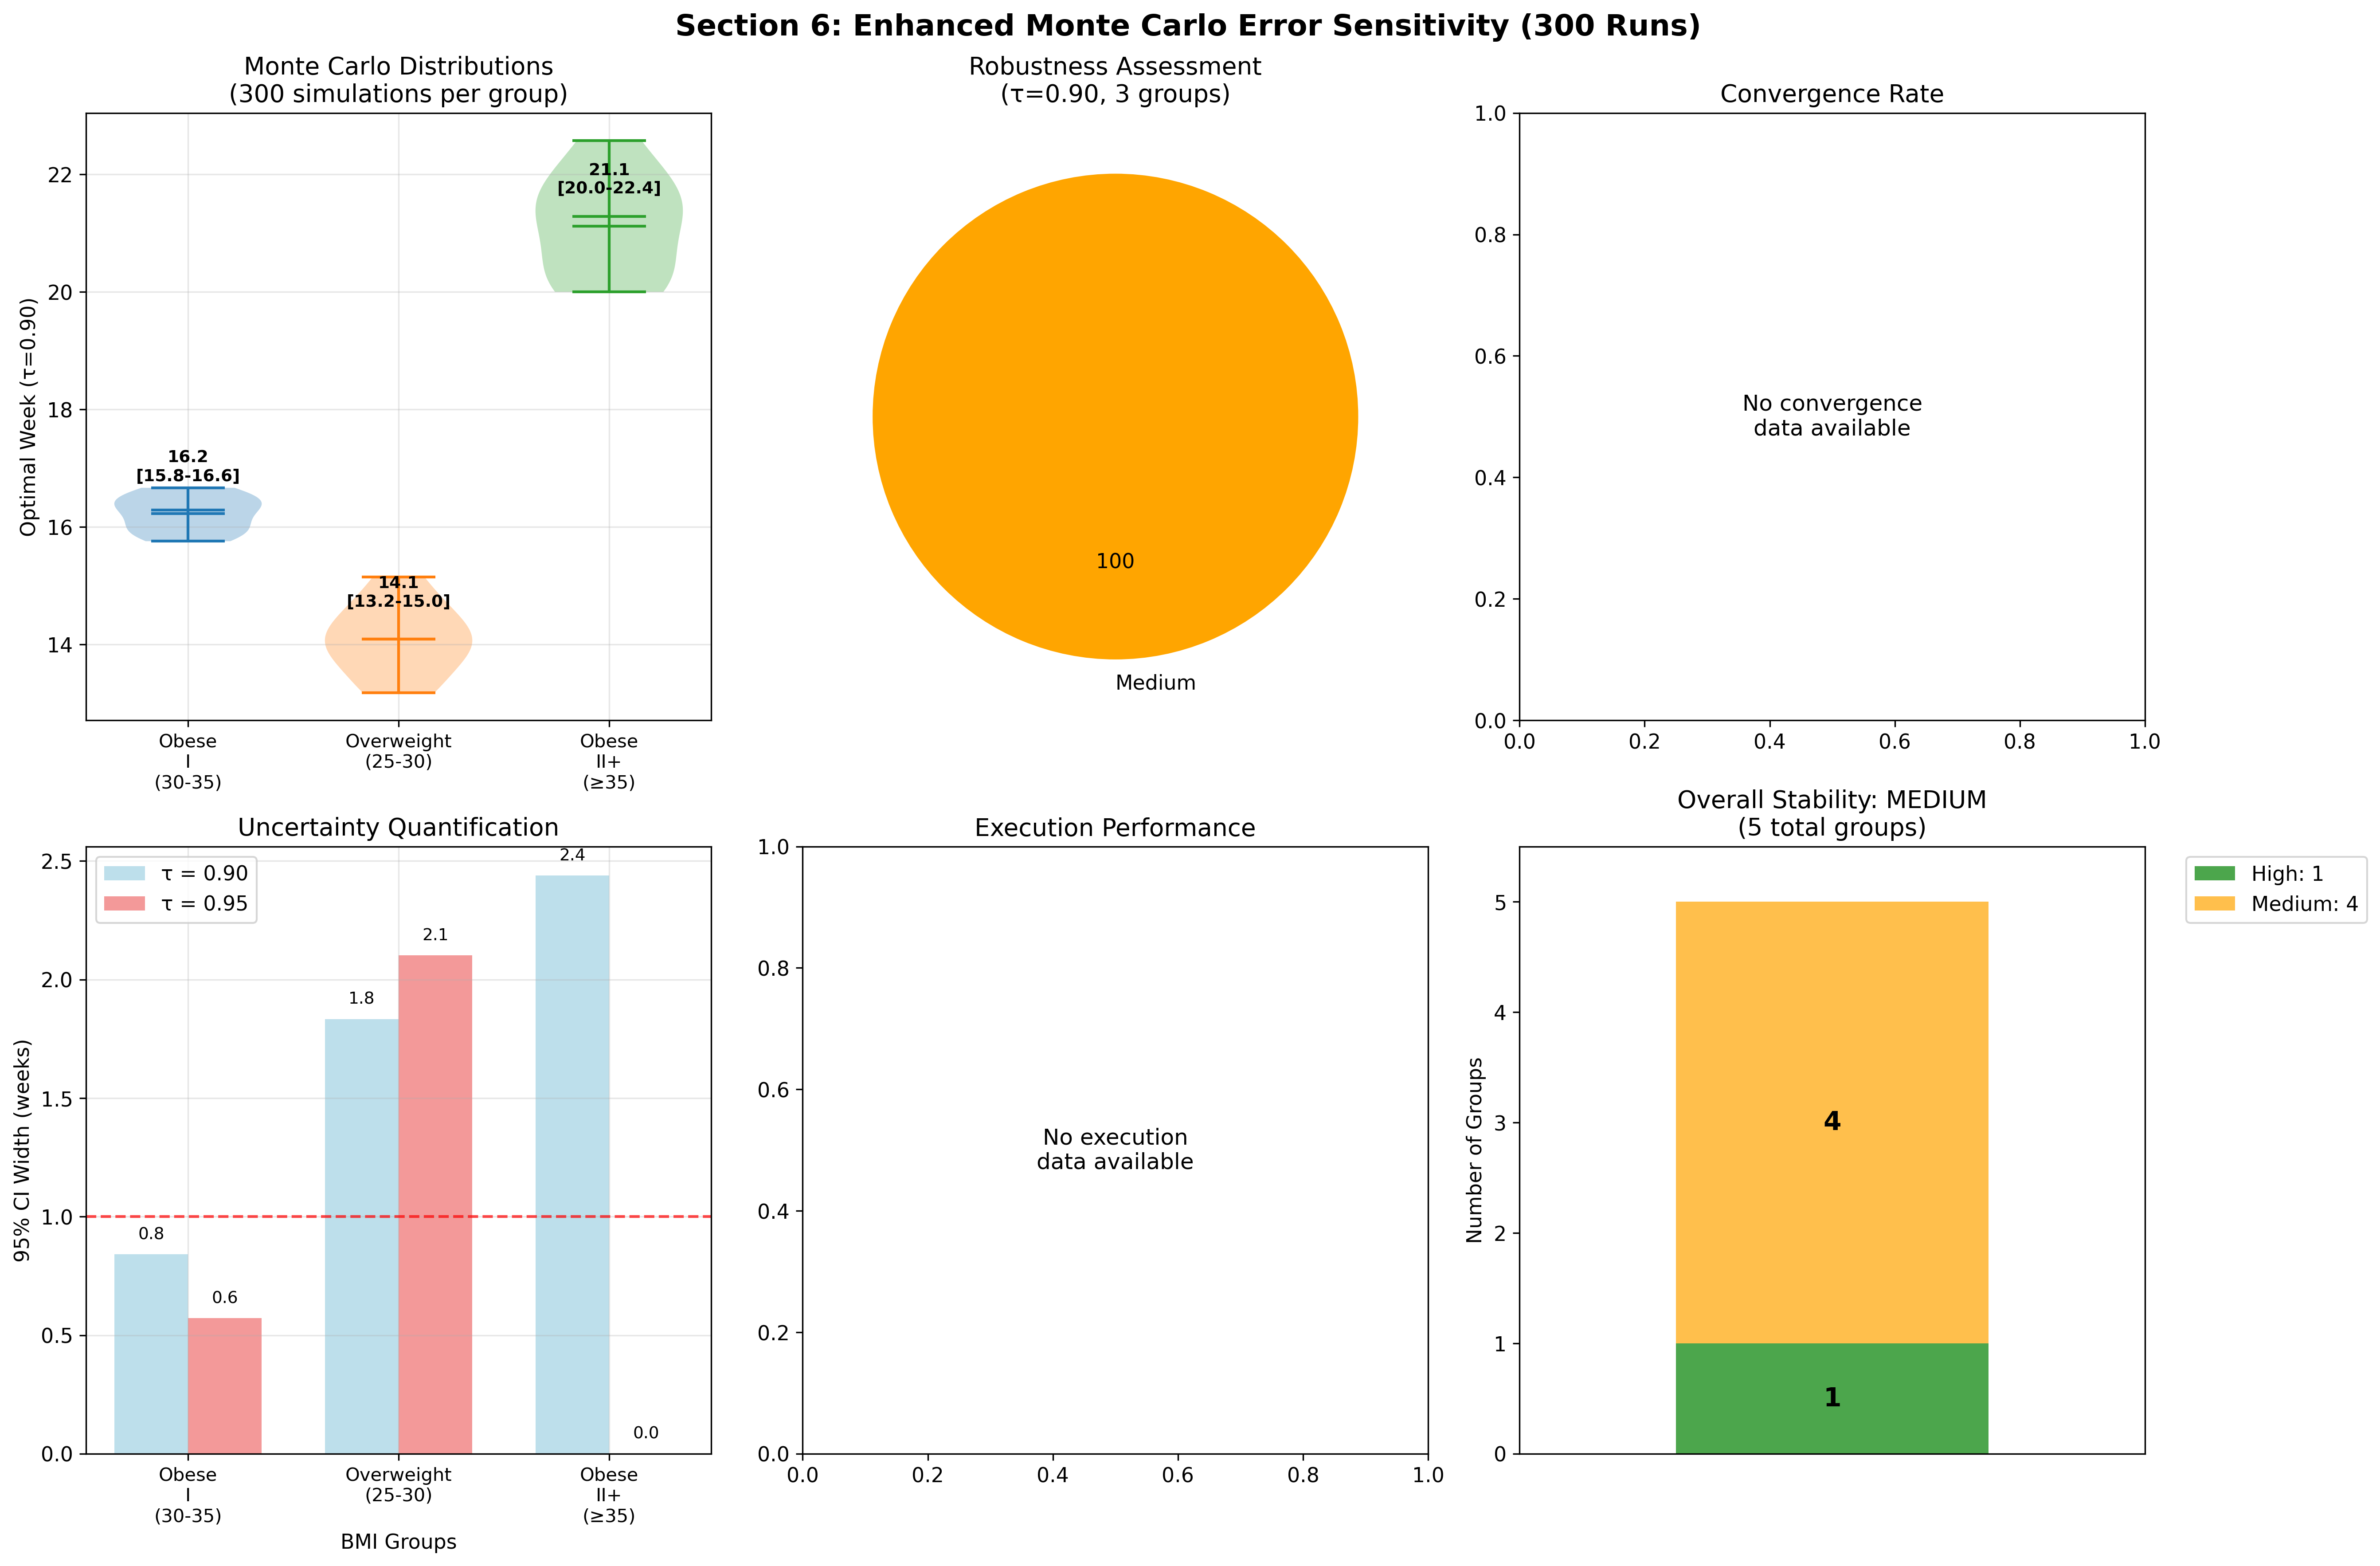
\includegraphics[width=\linewidth]{output/figures/p3_section6_monte_carlo_analysis.png}
  \caption{Monte Carlo 稳健性评估}
\end{subfigure}
\caption{问题三综合图示套件。(A) 不同AFT模型的AIC比较,支持Extended Weibull-AFT。 (B) Turnbull非参数曲线与AFT拟合曲线对比,显示一致性良好。(C) 各CART-BMI分组的生存曲线,高BMI组达标时间显著延迟。(D) $w^{*}_{0.90}$ 的MC模拟分布,高BMI组不确定性更大。}
\label{fig:p3_suite}
\end{figure}

\subsubsection{小结}
本节针对问题三,构建了一个综合考量个体差异、测量误差与删失结构的 AFT 策略框架。通过系统的模型比较,我们确定 Extended Weibull-AFT 模型为最优选择,但需注意统计功效有限(事件/协变量比仅3.7)。通过与非参数方法的对比、Bootstrap稳定性检验(50次重抽样)和Monte-Carlo模拟(300次运行),在一定假定下验证了模型的适用性。在临床实施层面,我们基于数据驱动的 CART 四分组(CART\_G1-G4),为每个 BMI 区间提供了在 90\% 和 95\% 置信水平下的``最早安全孕周''建议(表~\ref{tab:p3_policy_revised})。综合分析指出高 BMI 组别需采取更保守的时点策略,以确保检测的可靠性,从而在有限的统计功效下实现``尽早-稳健-简洁''的多目标风险最小化。

\subsection{问题四的建模与求解}

\subsubsection{问题分析}
本题针对女胎样本(母体与胎儿均不携带 Y 染色体),以 21/18/13 号染色体非整倍体(AB 列)为金标准标注,综合利用全基因组计数型 NIPT 的统计特征与实验质控指标,对“是否存在染色体异常”进行二分类建模。与男胎问题不同,本题无法借助 Y 信号,需在(i)多维统计信号弱、(ii)类别极度不均衡(阳性$\approx 10\%$)、(iii)实验因素(如 GC 偏好、测序深度、重复率等)产生噪声的条件下,获得兼具\emph{稳健性}(低假阳性率)与\emph{可解释性}(重要特征可回溯到具体染色体/质控项)的判定模型。

\subsubsection{特征构造与数据处理}
设样本数为 $n$,构造特征矩阵 $X\in\mathbb{R}^{n\times p}$、标签 $y\in\{0,1\}^n$(1 表示非整倍体阳性)。在数据清洗与标准化后,最终用于训练/验证/测试的样本划分为:训练集 $216$、校准集 $24$、测试集 $60$,测试集阳性率为 $10\%$。

\paragraph{特征集合}
\[
X=\big[\underbrace{Z_{13},Z_{18},Z_{21},Z_X}_{\text{染色体Z值}},\underbrace{GC_{\text{global}},GC_{13},GC_{18},GC_{21}}_{\text{GC含量}},\underbrace{\texttt{reads},\texttt{map\_ratio},\texttt{dup\_ratio},\texttt{unique\_reads},\texttt{uniq\_rate}}_{\text{测序深度/重复/唯一比对率}},\underbrace{\text{BMI},\text{age},\text{weeks}}_{\text{临床变量}},\underbrace{\texttt{max\_Z},\mathbb{I}(|Z_{13}|\!\ge3),\mathbb{I}(|Z_{18}|\!\ge3),\mathbb{I}(|Z_{21}|\!\ge3)}_{\text{统计汇总/指示量}}\big].
\]
其中 $\texttt{max\_Z}=\max\{|Z_{13}|,|Z_{18}|,|Z_{21}|,|Z_X|\}$;指示量 $\mathbb{I}(|Z_k|\!\ge3)$ 刻画传统阈值法的“可疑异常”标记。除去计数型变量外,所有连续特征在训练/校准/测试三个子集上以训练集统计量进行同分布标准化。额外的相关性分析显示 GC 含量与孕周、BMI、目标信号的皮尔逊相关系数接近 0(例如 $r\approx-0.001$ 与 $p\approx0.978$;图中给出三组相关系数与 $p$ 值),因此将 GC 项视作混杂控制变量纳入而不过度正则其影响。

\paragraph{类别不平衡处理} 采用类权重而非过采样:将损失函数中的阳性样本权重设定为 $\texttt{scale\_pos\_weight}\approx\frac{N_{\text{neg}}}{N_{\text{pos}}}=8.82$。

\subsubsection{模型的建立}
记 $f_\Theta:\mathbb{R}^p\!\to\!\mathbb{R}$ 为由 $M$ 棵 CART 弱学习器加性组成的梯度提升树(XGBoost):
\[
f_\Theta(x)=\sum_{m=1}^{M} g_m(x),\qquad g_m\in\mathcal{G}, 
\]
输出概率
\[
\hat{p}(x)=\sigma\!\big(f_\Theta(x)\big)=\frac{1}{1+e^{-f_\Theta(x)}},\quad \hat{y}=\mathbb{I}\{\hat{p}(x)>\tau\}.
\]
训练时最小化带类权重的对数损失并加入 $L_1/L_2$ 正则:
\[
\min_{\Theta}\ \sum_{i=1}^{n}w_{y_i}\,\ell\!\big(y_i,\hat{p}(x_i)\big)
+\lambda_1\|\Theta\|_{1}+\lambda_2\|\Theta\|_{2}^{2},\quad 
\ell(y,p)=-\big[y\log p+(1-y)\log(1-p)\big],
\]
其中 $w_{1}=\texttt{scale\_pos\_weight}=8.82,\ w_{0}=1$。

\subsubsection{模型训练与验证}
采用“训练/校准/测试”三分法:先在训练集进行带权训练并通过网格搜索选择超参数;随后使用\emph{独立校准集}($n=24$,阳性率 $8.33\%$)选择决策阈值 $\tau$,目标是在较低 FPR 下保留尽可能高的召回率。最终阈值确定为
\[
\tau^\star=0.524747\quad,
\]
在校准集达到召回率 $1.0$。概率输出的\emph{可靠性}通过校准曲线与 Brier 分数评估,详细见图 \ref{fig:p4_calib} 与表 \ref{tab:p4_metrics}。

\subsubsection{模型评价与对比}
在\emph{严格保留的测试集}($n=60$,阳性 $6$、阴性 $54$)上,基于 $\tau^\star$ 的性能如下:
\begin{itemize}
\item 混淆矩阵:$\begin{bmatrix}\text{TN}&\text{FP}\\ \text{FN}&\text{TP}\end{bmatrix}=\begin{bmatrix}53&1\\4&2\end{bmatrix}$;
\item 主要指标:准确率 $0.917$,精确率(PPV)$0.667$,召回率(灵敏度)$0.333$,特异度 $0.981$,FPR $0.019$,F1 $0.444$,ROC-AUC $0.806$,PR-AUC $0.481$,Brier 分数 $0.088$,NPV $0.930$;
\item 概率分布、ROC/PR 曲线与混淆矩阵见图 \ref{fig:p4_dashboard}。
\end{itemize}

为凸显阈值控制对“误报成本”的价值,我们还给出一个“高召回基线”:其召回率虽为 $1.0$,但 FPR 上升到 $0.370$($\text{FP}=20$)。相比之下,本文最终阈值将 FPR 压低至 $0.019$,代价是召回下降至 $0.333$,体现了临床筛查中“优先控制误报”的取舍。

\paragraph{特征重要性与可解释性}
XGBoost 的增益重要性与图 \ref{fig:p4_importance})前五名为:
\[
\texttt{max\_Z}(16.6\%),\ \texttt{Z18\_indicator}(7.6\%),\ \texttt{age}(5.7\%),\ Z_{18}(5.2\%),\ \texttt{uniq\_rate}(5.2\%).
\]
这与临床直觉一致:\emph{统计偏离最显著的染色体}(\texttt{max\_Z})与\emph{经典阈值指示量}($|Z_{18}|\!\ge3$ 等)对阳性判定贡献最大;测序深度与唯一比对率(\texttt{reads}/\texttt{uniq\_rate})反映技术波动;BMI、年龄等母体因素提供额外风险分层。GC 相关特征($GC_{\cdot}$)的重要性较低($2.9$--$3.8\%$),与其低相关性分析相符。
\begin{table}[!t]
\centering
\caption{女胎异常判定模型的测试集指标($\tau=0.524747$)}\label{tab:p4_metrics}
\begin{tabular}{lcccccccccc}
\hline
Acc & PPV & Rec & Spec & FPR & F1 & ROC-AUC & PR-AUC & Brier & NPV & $n$ \\
\hline
0.917 & 0.667 & 0.333 & 0.981 & 0.019 & 0.444 & 0.806 & 0.481 & 0.088 & 0.930 & 60 \\
\hline
\end{tabular}
\end{table}

\begin{figure}[!t]
\centering
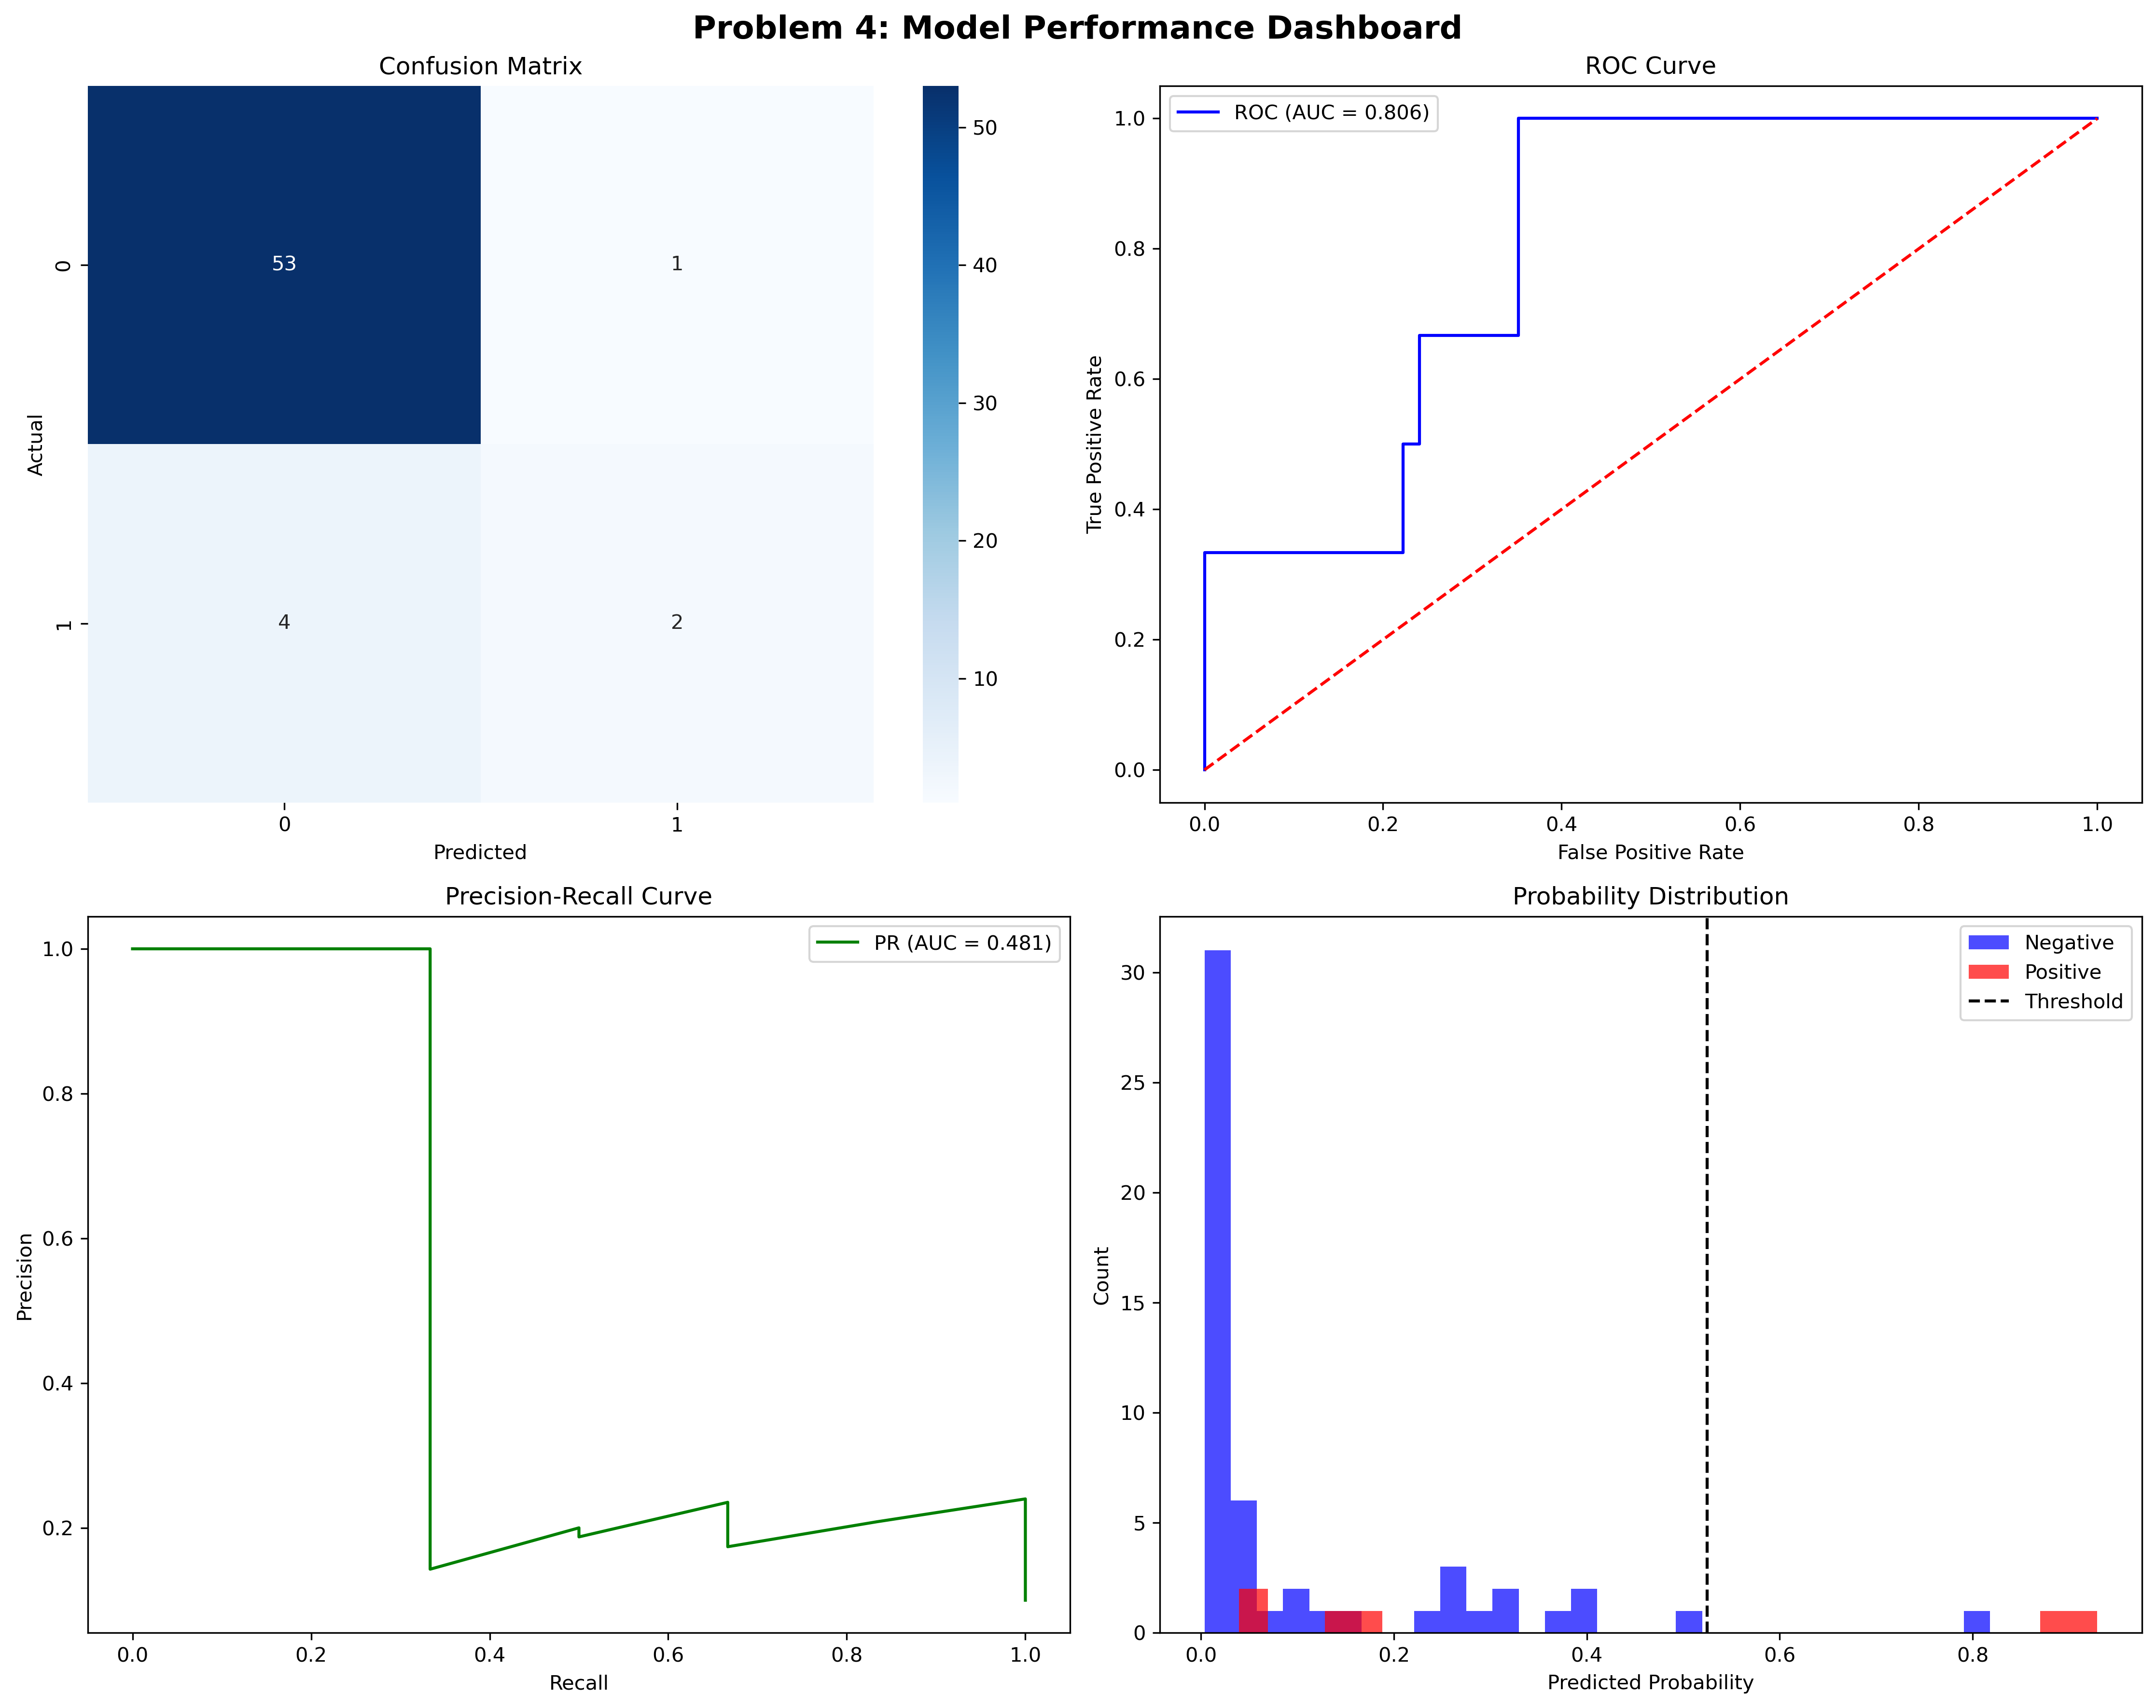
\includegraphics[width=0.95\linewidth]{output/figures/p4_final_model_dashboard.png}
\caption{整体性能:混淆矩阵、ROC/PR 曲线与预测概率分布。}
\label{fig:p4_dashboard}
\end{figure}

\begin{figure}[!t]
\centering
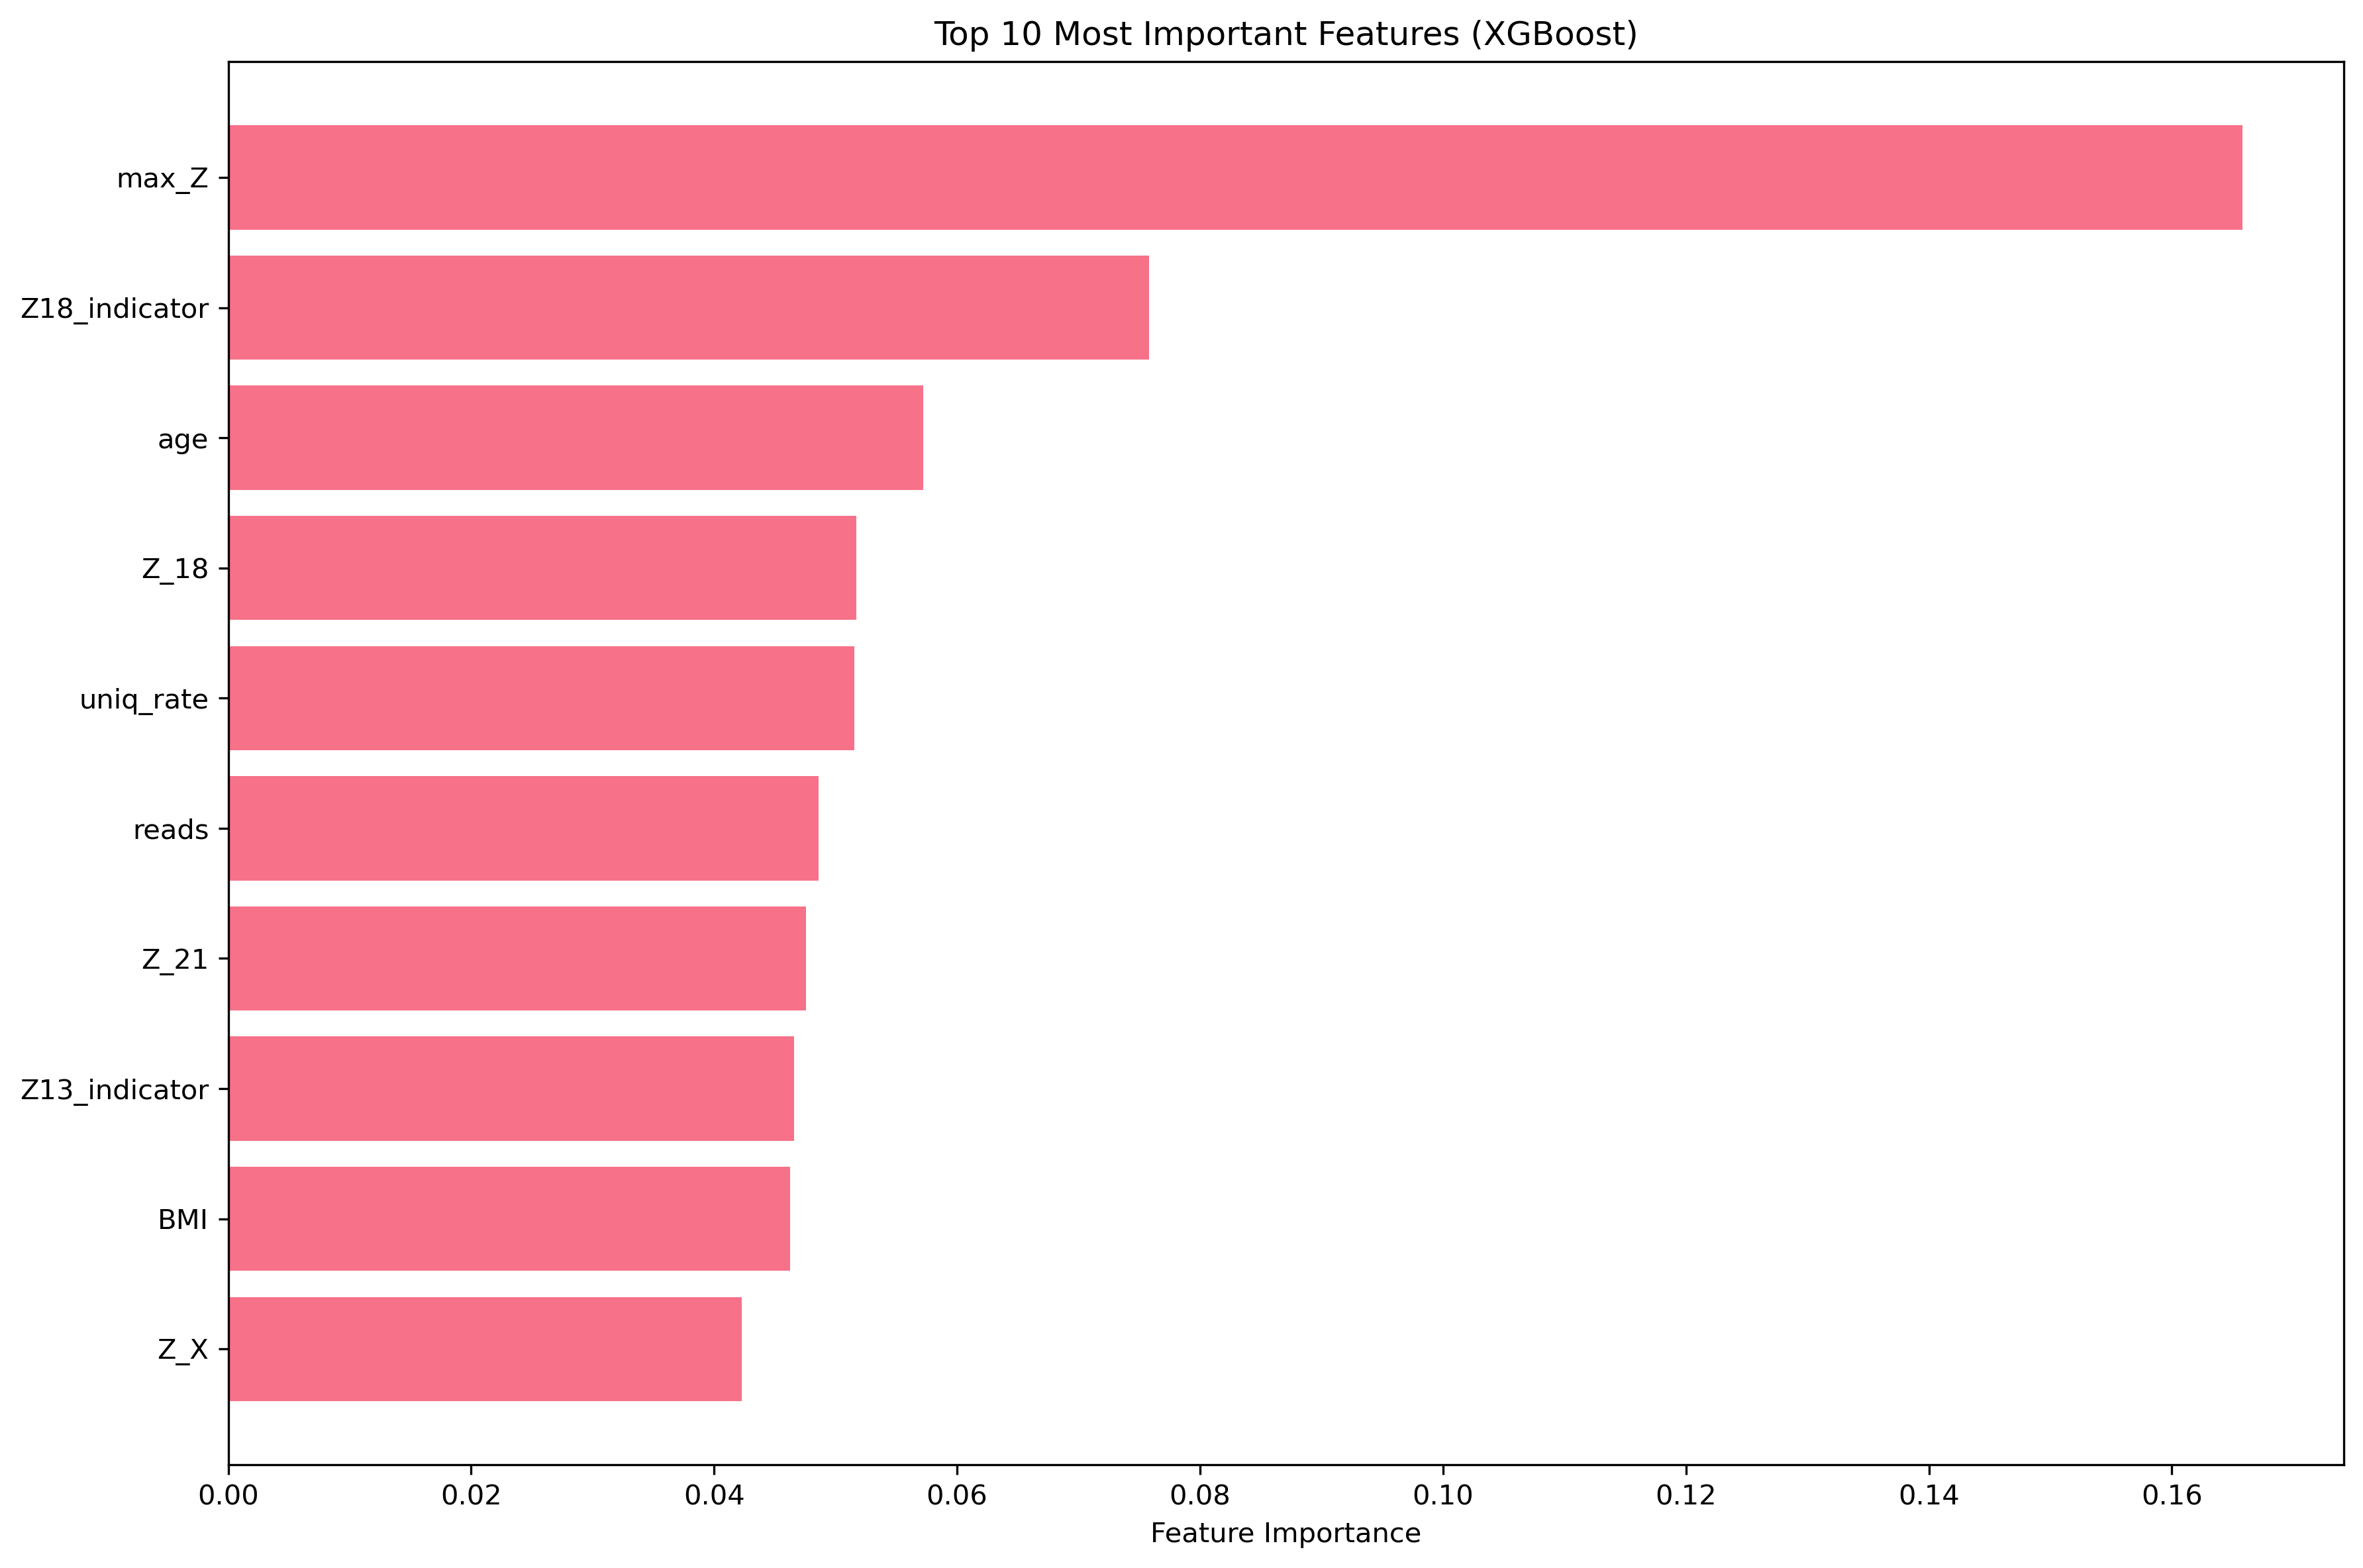
\includegraphics[width=0.85\linewidth]{output/figures/p4_feature_importance.png}
\caption{XGBoost 特征重要性(对应 \texttt{p4\_feature\_importance.png})。}
\label{fig:p4_importance}
\end{figure}

\begin{figure}[!t]
\centering
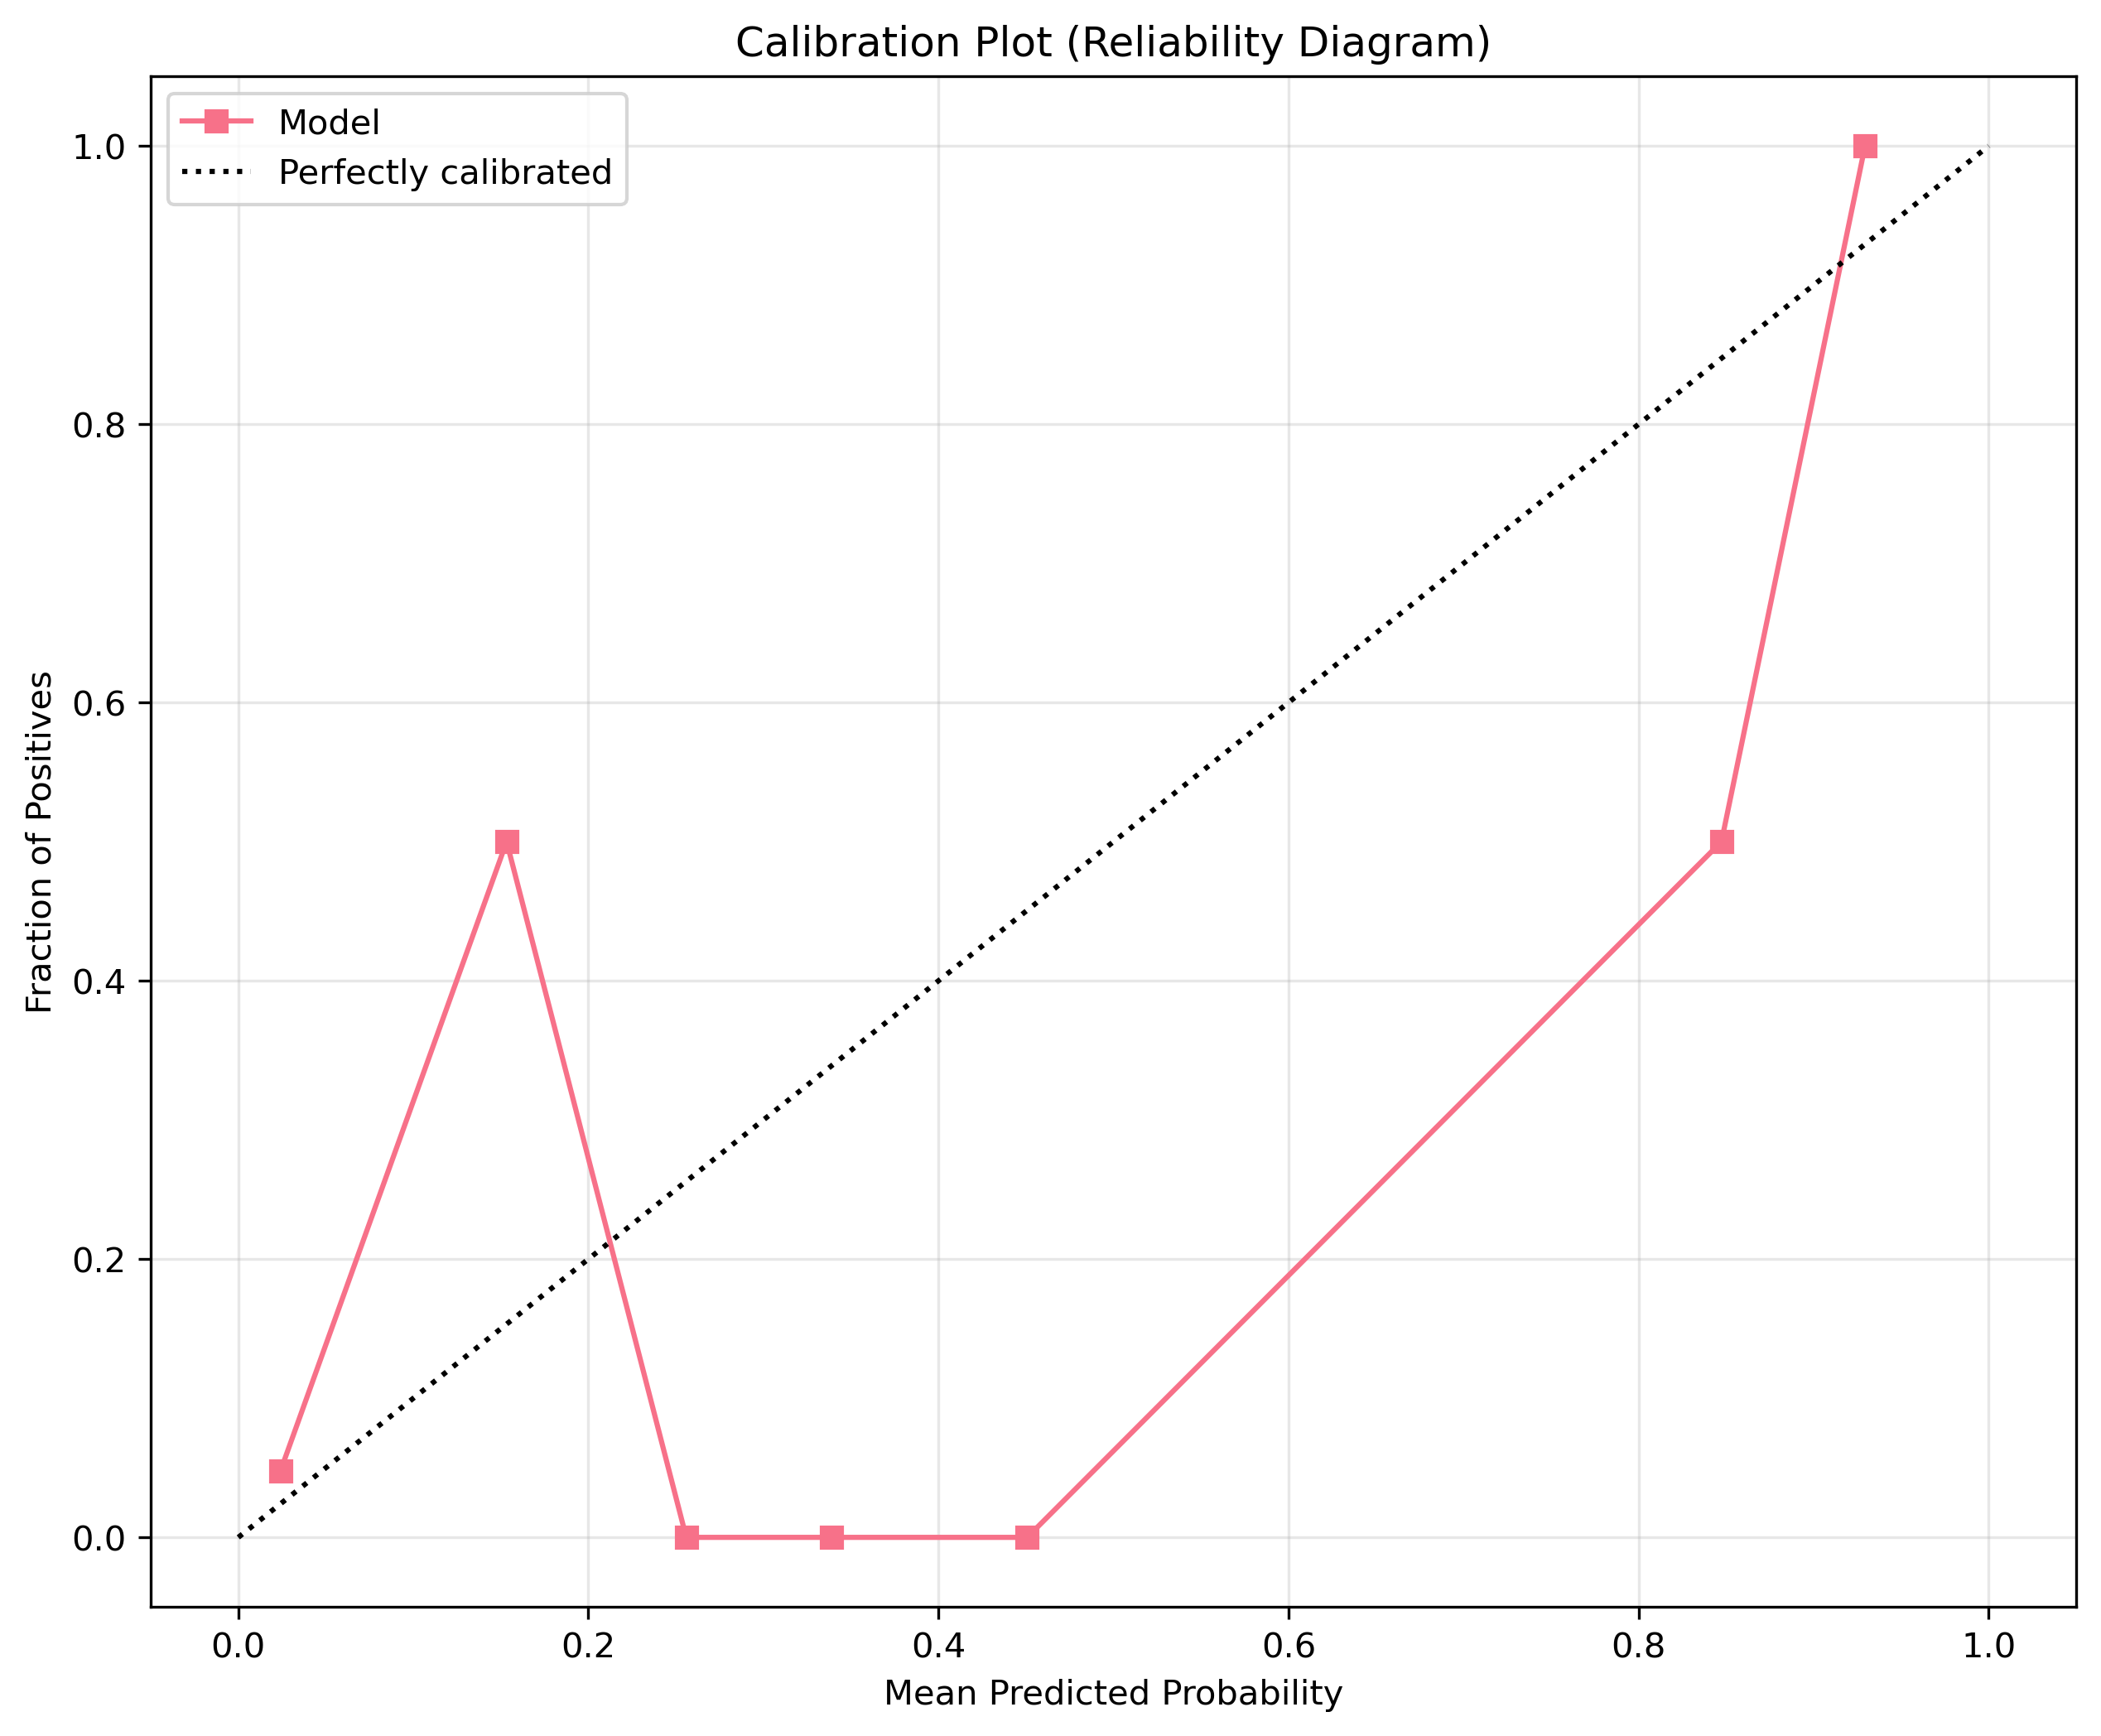
\includegraphics[width=0.7\linewidth]{output/figures/p4_calibration_curve.png}
\caption{概率校准评估(对应 \texttt{p4\_calibration\_curve.png})。}
\label{fig:p4_calib}
\end{figure}

\subsubsection{小结}
本文以 21/18/13 号染色体 AB 标注为金标准,围绕 Z 值、测序质控与母体临床变量构建了一个\emph{可解释}且\emph{低误报}的女胎异常判定框架。最终 XGBoost 模型在独立测试集上达到 ROC-AUC $0.806$、PR-AUC $0.481$,在 $\tau=0.524747$ 下实现 FPR $1.9\%$ 与准确率 $91.7\%$;重要性分析显示 \texttt{max\_Z} 与各染色体阈值指示量主导判别,GC 相关项影响较小。模型概率具有良好校准(Brier $0.088$)。局限性在于样本量与阳性例偏少导致召回率受限($33.3\%$);可在保持低 FPR 的前提下,通过(i)更丰富的片段长度/区域性偏差特征、(ii)集成校准与代价敏感阈值优化、(iii)多中心数据增广,进一步提升灵敏度。总体而言,所建模型为女胎样本的常见非整倍体筛查提供了统计上有效且临床可解释的证据基础。

\section{灵敏度分析}

灵敏度分析是评估模型稳定性和可靠性的关键环节。本研究通过鲁棒优化和动态调参两种方式,系统地检验了所建模型在关键假设、参数选择和外部扰动下的表现,以确保结论的稳健性。

\subsection{基于鲁棒优化的灵敏度分析}

为应对 NIPT 检测实践中不可避免的不确定性,我们引入了基于鲁棒优化的灵敏度分析框架。该框架主要关注由测量误差(measurement error)、数据删失(censoring)和分组策略(grouping)引入的潜在变异对模型结果的影响。

首先,在问题二和问题三的“最早安全孕周”$w_g^*$ 估计中,我们明确考虑了 Y 染色体浓度的测量误差。通过 \textbf{蒙特卡洛(Monte Carlo)模拟},我们在原始观测值上叠加一个服从正态分布的随机扰动($\epsilon \sim \mathcal{N}(0,\sigma^2)$),并在此基础上重复(300 次)构建区间删失数据集、重新拟合加速失效时间(Accelerated Failure Time, AFT)模型。这一过程生成了 $w_g^*$ 的经验分布,其置信区间(如 $95\%$ Monte Carlo IQR)直观地量化了在给定测量误差水平下,决策时点的不确定性。分析结果表明,尽管高 BMI 组的 $w_g^*$ 不确定性(置信区间宽度)显著增加,但对于大部分分组,推荐时点的估计在小幅度的测量扰动下是相对稳定的,证实了我们策略的鲁棒性。

其次,区间删失框架本身即是一种处理不确定性的鲁棒方法。它不依赖于精确的事件发生时间(FF 浓度首次达标),而是利用其所在的时间区间 $(L,R]$ 进行建模,有效适应了临床随访数据的非精确性。我们在问题二中对比了参数化的 AFT 模型与非参数的 Turnbull 估计,两者在核心临床窗口内(12.0--24.7 周)的生存曲线高度一致(Mean Absolute Error, MAE $\approx 0.0141$),这表明 AFT 模型的分布假设是合理的,其结论不受特定参数形式的严重束缚。

最后,在问题一的线性混合效应模型中,我们采用了异方差稳健标准误(heteroskedasticity-consistent standard errors),确保了在残差方差不齐的情况下,对孕周和 BMI 效应的统计推断依然可靠。

\subsection{基于动态调参的灵敏度分析}

动态调参的灵敏度分析旨在评估模型结果对关键超参数(hyperparameters)和决策阈值(thresholds)变化的敏感程度。

\paragraph{(1) 决策阈值的影响} 在问题二和问题三中,我们分别计算了在两种不同置信水平($\tau=0.90$ 和 $\tau=0.95$)下的推荐孕周 $w_g^*$。结果清晰地显示,当要求从 $90\%$ 提升至 $95\%$ 的达标概率时,推荐孕周显著后推,且对于极高 BMI 组,甚至出现了在观测窗口内无法达标(“Never”)的情况。这揭示了临床决策中“风险规避水平”与“检测时点”之间的定量权衡关系,表明我们的模型能够根据不同的风险偏好提供动态的、差异化的策略。

\paragraph{(2) 核心假设的敏感性} 在生存分析部分,我们比较了基于不同概率分布假设的 AFT 模型(Weibull-AFT vs log-logistic AFT)。尽管两者对 BMI 效应的定性结论一致,但 Weibull 模型在赤池信息准则(AIC)上表现更优,故被选为最终模型。这一对比过程确保了我们的选择是数据驱动的,而非依赖于单一的先验假设。

\paragraph{(3) 模型结构参数的调整} 我们评估了模型结构参数的调整对结果的影响。例如,在问题一中,我们通过比较不同自由度的自然样条(natural splines)模型,最终确定 $\mathrm{df}=3$ 是描述孕周非线性效应的最佳选择。在问题四的女胎异常检测中,XGBoost 模型的超参数(如树的最大深度 \texttt{max\_depth}、学习率 \texttt{eta} 等)均通过系统的网格搜索与交叉验证确定,以平衡模型的拟合能力与泛化性能。这些分析共同验证了我们所选模型结构在各自问题背景下的合理性与最优性。

\section{模型评价与推广}

\subsection{模型的优点}

本研究建立的系列模型具有以下突出优点:
\begin{itemize}
    \item \textbf{可解释性与临床对齐}:模型并非“黑箱”,且与临床逻辑紧密结合。问题一的混合效应模型清晰量化了孕周与 BMI 对 Y 浓度的影响;问题二与问题三的 AFT 模型提供了直观的时间比(time ratio)解释,直接关联到不同 BMI 分组下 FF 浓度达标的“加速/减速”效应;问题四的 XGBoost 模型通过特征重要性(feature importance)明确了 Z 值、年龄、测序质量等指标在异常判定中的贡献,符合临床直觉。
    \item \textbf{多层次稳健性验证}:综合运用了多种验证方法,包括(1)问题二中的 5 折交叉验证(5-fold cross-validation);(2)问题二、三中参数化 AFT 模型与非参数 Turnbull 估计的一致性验证;(3)针对测量误差的蒙特卡洛模拟;(4)问题四中严格划分训练集、校准集(calibration set)与测试集(test set),并对概率进行了校准评估(Brier score $=0.088$),确保结论在不同数据子集与扰动下的稳定性。
    \item \textbf{对复杂数据结构的有效处理}:问题一的线性混合效应模型有效处理了同一孕妇重复测量(repeated measures)导致的组内相关;问题二、三将时点选择问题转化为\textbf{区间删失(interval censoring)}的生存分析问题,适配非精确事件时间;问题四通过类别加权(class weighting)缓解了阳性样本稀疏(class imbalance)带来的挑战。
\end{itemize}

\subsection{模型的缺点}

尽管模型表现优良,仍存在以下局限:
\begin{itemize}
    \item \textbf{数据来源的局限性}:数据主要来自“高 BMI”孕妇群体,可能导致在低或正常 BMI 人群中的泛化能力受限。参数与分组阈值可能反映特定人群特征,直接迁移需谨慎。
    \item \textbf{删失数据与统计功效}:问题三中重度左删失比例高(约 $85.0\%$),虽可被模型处理,但可用于精确估计事件时间分布的信息相对较少。引入多协变量后,events-per-variable 偏低,可能影响参数估计稳定性与统计功效(statistical power)。
    \item \textbf{极端子群的可靠性}:对部分极端子群,预测可靠性下降。例如问题二中 BMI 极高组(CART\_G6)在 $95\%$ 置信度下无法在临床窗口内达标,提示该区间的预测能力有限。问题四中由于非整倍体异常发生率极低,即便总体表现良好,识别罕见异常类型时的灵敏度(召回率)仍需提升(测试集召回率为 $0.333$)。
\end{itemize}

\subsection{模型的推广}

本研究的建模框架具有良好推广潜力:
\begin{itemize}
    \item \textbf{更广泛的数据集}:将 AFT 生存模型与 XGBoost 分类模型应用于更大、更异质的人群(不同 BMI、种族、医疗中心),以验证并提升外部效度(external validity),形成更具普适性的临床决策规则。
    \item \textbf{拓展临床场景}:时间到事件分析框架可迁移至其他需确定最佳检测/干预时点的任务(如其他血清生物标志物的动态监测)。女胎异常检测框架可纳入更多特征(如胎儿 DNA 片段长度分布),以检测更多遗传异常(如微缺失/微重复)。
    \item \textbf{与临床决策支持系统(CDSS)集成}:BMI 分组策略、推荐孕周表与女胎异常风险评分可转化为临床工具,并与医院信息系统集成,提供实时、个体化的 NIPT 时点建议与风险评估。
    \item \textbf{模型迭代与优化}:随数据累积,可引入更先进的算法(如深度生存模型)或多组学数据,进一步提升预测精度与个体化水平。
\end{itemize}

\section{结论与展望}

本研究基于真实 NIPT 数据,围绕临床核心问题,构建了数据驱动、可解释且经充分验证的综合建模框架。首先,通过包含自然样条与随机效应的线性混合模型,精确刻画了男胎 Y 染色体浓度与孕周(非线性正相关)及 BMI(线性负相关)之间的量化关系。其次,将 NIPT 最佳时点选择问题创新性转化为区间删失的生存分析问题,采用 Weibull-AFT 模型并结合 CART 算法,为不同 BMI 分层的孕妇群体提供了风险最小化的“最早安全孕周”策略。最后,针对女胎,构建了基于 XGBoost 的分类模型,综合染色体 Z 值、测序质量与母体临床特征,实现了低误报率(FPR $=1.9\%$)的精准筛查。

展望未来,可在以下方面深化与拓展:(1)融合生存分析与前沿机器学习方法(如随机生存森林、深度学习)以捕捉更高维复杂非线性;(2)针对女胎异常检测的极度类不平衡,研究代价敏感学习与集成异常检测方法,在保持低假阳性率的同时提升召回率;(3)持续优化概率校准,引入动态校准机制,确保不同时间与人群中的预测可靠性。

综上,本研究为优化 NIPT 临床实践提供了可量化的决策支持工具,并展示了统计学严谨性与机器学习灵活性相结合的建模思路。随着研究深入与数据丰富,该框架有望进一步推动精准产前诊断与母婴健康水平的提升。


% 参考文献
\begin{thebibliography}{99}

\bibitem{Lu2019cfDNA}
Lu, Y. \emph{et al.}
\newblock Sequencing of short cfDNA fragments in NIPT improves fetal fraction with higher maternal BMI and early gestational age.
\newblock {\em American Journal of Translational Research}, 2019.
\newblock \url{https://pmc.ncbi.nlm.nih.gov/articles/PMC6684886/}.

\bibitem{Xie2023FetalFraction}
Xie, X. \emph{et al.}
\newblock Maternal and fetal factors influencing fetal fraction: analysis of 153,306 women.
\newblock {\em Frontiers in Pediatrics}, 2023.
\newblock DOI: \href{https://doi.org/10.3389/fped.2023.1066178}{10.3389/fped.2023.1066178}.

\bibitem{Zhao2021LowFF}
Zhao, J. \emph{et al.}
\newblock Multivariate modeling for prediction of low fetal fraction before NIPT.
\newblock {\em Proceedings of the Royal Society B}, 2021.
\newblock \url{https://pmc.ncbi.nlm.nih.gov/articles/PMC10358597/}.

\bibitem{Yang2018SVM}
Yang, J. \emph{et al.}
\newblock Improving NIPT trisomy calling by SVM.
\newblock {\em PLOS ONE}, 13(12):e0207840, 2018.
\newblock \url{https://journals.plos.org/plosone/article?id=10.1371/journal.pone.0207840}.

\bibitem{Muzzey2020BMI}
Muzzey, D. \emph{et al.}
\newblock NIPS for high BMI: customized WGS workflow impact.
\newblock {\em Prenatal Diagnosis}, 40(3):333--341, 2020.

\bibitem{许显峰2022ML}
许显峰, 刘媛, 赵丽.
\newblock 机器学习评估 USM 联合 NIPT 诊断胎儿染色体异常的价值.
\newblock {\em 数学的生物科学与工程}, 19(4):4260--4276, 2022.

\bibitem{妇幼保健医学2019指南}
《无创产前检测临床应用相关指南解读》.
\newblock {\em 妇幼保健医学}, 34(1), 2019.

\bibitem{Claude}
Claude, Claude-4-Sonnet, Anthropic, 2025-05-22.

\bibitem{GPT5}
GPT-5, GPT-5, OpenAI, 2025-08-07.

\end{thebibliography}

\newpage
\section{论文附录}

\subsection{支撑材料文件列表}

本论文的建模与分析过程中使用了以下支撑材料,所有文件均可运行且结果与论文一致:

\subsubsection{数据文件}
\begin{itemize}
    \item \texttt{src/attachment.xlsx} - 竞赛原始数据文件
    \item \texttt{src/data/data.xlsx} - 预处理后的分析数据
    \item \texttt{output/data/clean\_dataset\_prob1.csv} - 问题一清洗后数据集
    \item \texttt{output/data/prob2\_clean\_dataset.csv} - 问题二清洗后数据集
\end{itemize}

\subsubsection{源程序代码文件}
\begin{itemize}
    \item \texttt{src/main.py} - 主程序入口
    \item \texttt{src/config/settings.py} - 配置文件
    \item \texttt{src/data/loader.py} - 数据加载模块
    \item \texttt{src/utils/statistics.py} - 统计分析工具
    \item \texttt{src/utils/visualization.py} - 可视化工具
\end{itemize}

\paragraph{问题一相关代码:}
\begin{itemize}
    \item \texttt{src/analysis/problem1/correlation\_analysis.py} - 相关性分析模块
    \item \texttt{src/notebooks/00\_prob1\_preprocessing.ipynb} - 数据预处理笔记本
    \item \texttt{src/notebooks/01\_prob1.ipynb} - 问题一建模与分析笔记本
\end{itemize}

\paragraph{问题二相关代码:}
\begin{itemize}
    \item \texttt{src/analysis/problem2/data\_preprocessing.py} - 数据预处理模块
    \item \texttt{src/analysis/problem2/survival\_analysis.py} - 生存分析模块
    \item \texttt{src/analysis/problem2/bmi\_grouping.py} - BMI分组策略模块
    \item \texttt{src/analysis/problem2/monte\_carlo.py} - 蒙特卡洛模拟模块
    \item \texttt{src/analysis/problem2/validation.py} - 模型验证模块
    \item \texttt{src/analysis/problem2/ml\_baseline.py} - 机器学习基准模型
    \item \texttt{src/models/aft\_models.py} - 加速失效时间模型
    \item \texttt{src/notebooks/02\_prob2.ipynb} - 问题二建模与分析笔记本
\end{itemize}

\paragraph{问题三相关代码:}
\begin{itemize}
    \item \texttt{src/analysis/problem3/data\_preprocessing.py} - 数据预处理模块
    \item \texttt{src/analysis/problem3/survival\_analysis.py} - 生存分析模块
    \item \texttt{src/analysis/problem3/bmi\_grouping.py} - BMI分组策略模块
    \item \texttt{src/analysis/problem3/monte\_carlo.py} - 蒙特卡洛模拟模块
    \item \texttt{src/analysis/problem3/validation.py} - 模型验证模块
    \item \texttt{src/notebooks/03\_prob3.ipynb} - 问题三建模与分析笔记本
\end{itemize}

\paragraph{问题四相关代码:}
\begin{itemize}
    \item \texttt{src/analysis/problem4/data\_preprocessing.py} - 数据预处理模块
    \item \texttt{src/analysis/problem4/preprocessing\_transformers.py} - 预处理转换器
    \item \texttt{src/models/problem4\_models.py} - 问题四主要模型
    \item \texttt{src/models/problem4\_improvements.py} - 模型改进版本
    \item \texttt{src/models/problem4\_enhanced\_triage.py} - 增强筛查模型
    \item \texttt{src/models/problem4\_precision\_triage.py} - 精确筛查模型
    \item \texttt{src/models/problem4\_stable\_recall.py} - 稳定召回模型
    \item \texttt{run\_problem4\_pipeline.py} - 问题四流水线脚本
    \item \texttt{run\_problem4\_clinical\_validation.py} - 临床验证脚本
    \item \texttt{use\_trained\_model.py} - 训练模型使用脚本
\end{itemize}

\subsubsection{工具和诊断代码}
\begin{itemize}
    \item \texttt{src/utils/diagnostics/run\_all.py} - 诊断工具主程序
    \item \texttt{src/utils/diagnostics/gc\_correlation.py} - GC含量相关性分析
    \item \texttt{src/utils/diagnostics/filter\_impact.py} - 过滤影响分析
    \item \texttt{src/utils/diagnostics/selection\_bias.py} - 选择偏差分析
    \item \texttt{run\_diagnostics.py} - 综合诊断脚本
\end{itemize}

\subsubsection{结果输出文件}
\begin{itemize}
    \item \texttt{output/results/} - 包含所有分析结果的CSV和JSON文件(46个CSV文件,4个JSON文件,2个PKL文件)
    \item \texttt{output/figures/} - 包含论文中所有图表的PNG文件(27个图像文件)
    \item \texttt{output/clinical\_validation/} - 临床验证结果文件
\end{itemize}

\subsubsection{AI工具使用文档}
\begin{itemize}
    \item \texttt{AI工具使用详情.pdf} - AI工具使用的详细记录文档,包含使用目的、交互记录、采纳和修改情况
\end{itemize}

\subsection{软件环境与运行说明}

\subsubsection{环境要求}
本论文所有程序基于Python 3.8+环境开发,完整的依赖列表见项目根目录下的\texttt{requirements.txt}文件。

\subsubsection{运行方式}
\begin{enumerate}
    \item 环境配置:使用conda创建虚拟环境并安装依赖
    \begin{verbatim}
    conda create -n cumcm-env python=3.8
    conda activate cumcm-env
    pip install -r requirements.txt
    \end{verbatim}
    
    \item 数据预处理与分析:
    \begin{verbatim}
    # 运行完整分析流程
    python src/main.py
    
    # 运行问题四流水线
    python run_problem4_pipeline.py
    
    # 运行临床验证
    python run_problem4_clinical_validation.py
    
    # 运行诊断工具
    python run_diagnostics.py
    \end{verbatim}
    
    \item 交互式分析:使用Jupyter Notebook
    \begin{verbatim}
    jupyter notebook src/notebooks/
    \end{verbatim}
\end{enumerate}

\subsection{AI工具使用说明}

\subsubsection{AI工具使用概况}
本研究在代码实现、算法优化和部分技术文档编写过程中使用了AI辅助工具。所有AI生成的内容均经过人工审查、验证和修改,确保其准确性和适用性。

\subsubsection{使用的AI工具}
\begin{itemize}
    \item \textbf{Claude (Claude-4-Sonnet)}~\cite{Claude}:用于代码生成、算法实现建议和技术问题解答
    \item \textbf{GPT-5}~\cite{GPT5}:用于代码自动补全和函数实现辅助
\end{itemize}

\subsubsection{具体使用环节}
\begin{enumerate}
    \item \textbf{数据预处理代码优化}:使用AI工具优化数据清洗和转换逻辑
    \item \textbf{统计模型实现}:在混合效应模型、生存分析模型的Python实现中获得算法建议
    \item \textbf{机器学习模型调优}:在XGBoost参数调优和交叉验证实现中使用AI辅助
    \item \textbf{可视化代码生成}:部分图表绘制代码通过AI工具生成并人工修改
    \item \textbf{代码结构优化}:使用AI工具建议改进代码的模块化设计和错误处理
\end{enumerate}

\subsubsection{人工验证与修改}
所有AI生成的代码和建议均经过以下验证过程:
\begin{itemize}
    \item \textbf{逻辑验证}:确保算法逻辑正确,符合统计学和机器学习理论
    \item \textbf{结果验证}:运行代码并验证输出结果的合理性
    \item \textbf{性能测试}:测试代码的运行效率和稳定性
    \item \textbf{人工修改}:根据具体需求对AI生成的代码进行定制化修改
\end{itemize}

\subsubsection{AI工具使用详情文档}
详细的AI工具使用记录(包括Claude-4-Sonnet和GPT-5的关键交互记录、提示词与回复、采纳和修改情况)已整理为独立的PDF文档,文件名为"AI工具使用详情.pdf",包含在支撑材料中。

\subsection{声明}

本论文的所有分析均基于提供的原始数据,使用上述列出的完整、可运行的源程序代码实现。所有结果均可通过运行相应程序重现,确保了研究的可重复性和透明度。AI工具的使用仅限于代码实现辅助,核心的数学建模思路、统计分析方法和结论解释均为作者独立完成。

\end{document}